%============================================================================
% tento soubor pouzijte jako zaklad
% (c) 2008 Michal Bidlo
% E-mail: bidlom AT fit vutbr cz
%============================================================================
% kodovaní: iso-8859-2 (zmena prikazem iconv, recode nebo cstocs)
%----------------------------------------------------------------------------
% zpracování: make, make pdf, make desky, make clean
% připomínky posílejte na e-mail: bidlom AT fit.vutbr.cz
% vim: set syntax=tex encoding=latin2:
%============================================================================
\documentclass[english,cover]{fitthesis} % odevzdani do wisu - odkazy, na ktere se da klikat
%\documentclass[cover,print]{fitthesis} % pro tisk - na odkazy se neda klikat
%\documentclass[english,print]{fitthesis} % pro tisk - na odkazy se neda klikat
%      \documentclass[english]{fitthesis}
% * Je-li prace psana v anglickem jazyce, je zapotrebi u tridy pouzit 
%   parametr english nasledovne:
% \documentclass[english]{fitthesis}
% * Neprejete-li si vysazet na prvni strane dokumentu desky, zruste 
%   parametr cover

% zde zvolime kodovani, ve kterem je napsan text prace
% "latin2" pro iso8859-2 nebo "cp1250" pro windows-1250, "utf8" pro "utf-8"
%\usepackage{ucs}
\usepackage[utf8]{inputenc}
\usepackage[T1, IL2]{fontenc}
\usepackage{url}
\DeclareUrlCommand\url{\def\UrlLeft{<}\def\UrlRight{>} \urlstyle{tt}}

%zde muzeme vlozit vlastni balicky
\usepackage{feynmp}


% =======================================================================
% balíček "hyperref" vytváří klikací odkazy v pdf, pokud tedy použijeme pdflatex
% problém je, že balíček hyperref musí být uveden jako poslední, takže nemůže
% být v šabloně
\ifWis
\ifx\pdfoutput\undefined % nejedeme pod pdflatexem
\else
  \usepackage{color}
  \usepackage[unicode,colorlinks,hyperindex,plainpages=false,pdftex]{hyperref}
  \definecolor{links}{rgb}{0.4,0.5,0}
  \definecolor{anchors}{rgb}{1,0,0}
  \def\AnchorColor{anchors}
  \def\LinkColor{links}
  \def\pdfBorderAttrs{/Border [0 0 0] }  % bez okrajů kolem odkazů
  \pdfcompresslevel=9
\fi
\fi

%Informace o praci/projektu
%---------------------------------------------------------------------------
\projectinfo{
  %Prace
  project=SP,            %typ prace BP/SP/DP/DR
  year=2014,             %rok
  date=\today,           %datum odevzdani
  %Nazev prace
  title.cs={3D Rekonstrukce historických míst z obrázků na Flickru},  %nazev prace v cestine
  title.en={3D Reconstruction of Historic Landmarks from Flickr Pictures}, %nazev prace v anglictine
  %Autor
  author={Vojtěch Šimetka},   %jmeno prijmeni autora
  author.title.p=Bc., %titul pred jmenem (nepovinne)
  %author.title.a=PhD, %titul za jmenem (nepovinne)
  %Ustav
  department=UPGM, % doplnte prislusnou zkratku: UPSY/UIFS/UITS/UPGM
  %Skolitel
  supervisor= Ila Viorela Simona, %jmeno prijmeni skolitele
  supervisor.title.p=Ing.,   %titul pred jmenem (nepovinne)
  supervisor.title.a={Ph.D.},    %titul za jmenem (nepovinne)
  %Klicova slova, abstrakty, prohlaseni a podekovani je mozne definovat 
  %bud pomoci nasledujicich parametru nebo pomoci vyhrazenych maker (viz dale)
  %===========================================================================
  %Klicova slova
  keywords.cs={}, %klicova slova v ceskem jazyce
  keywords.en={}, %klicova slova v anglickem jazyce
  %Abstract
  abstract.cs={}, % abstrakt v anglickem jazyce
  abstract.en={}, % abstrakt v anglickem jazyce
  %Prohlaseni
  declaration={},
  %Podekovani (nepovinne)
  acknowledgment={} % nepovinne
}

%Abstrakt (cesky, anglicky)
%\abstract[cs]{Do tohoto odstavce bude zapsán výtah (abstrakt) práce v českém jazyce.}
%\abstract[en]{Do tohoto odstavce bude zapsán výtah (abstrakt) práce v anglickém jazyce.}

%Klicova slova (cesky, anglicky)
%\keywords[cs]{Sem budou zapsána jednotlivá klíčová slova v českém jazyce, oddělená čárkami.}
%\keywords[en]{Sem budou zapsána jednotlivá klíčová slova v anglickém jazyce, oddělená čárkami.}

%Prohlaseni
\declaration{Prohlašuji, že jsem tento semestrální projekt vypracoval samostatně pod vedením Ing. Ila Viorela Simona, Ph. D. a uvedl jsem všechny literární prameny a publikace, ze kterých jsem čerpal.}
%Další informace mi poskytli...
%Uvedl jsem všechny literární prameny a publikace, ze kterých jsem čerpal.}

%Podekovani (nepovinne)
%\acknowledgment{V této sekci je možno uvést poděkování vedoucímu práce a těm, kteří poskytli odbornou pomoc
%(externí zadavatel, konzultant, apod.).}

\begin{document}
  % Vysazeni titulnich stran
  % ----------------------------------------------
  \maketitle
  % Obsah
  % ----------------------------------------------
  \setcounter{tocdepth}{1}
  \tableofcontents
  
  % Seznam obrazku a tabulek (pokud prace obsahuje velke mnozstvi obrazku, tak se to hodi)
  % \listoffigures
  % \listoftables 

  % Text prace
  % ----------------------------------------------
  %=========================================================================

\chapter{Introduction}
This chapter describes the motivation leading to the presentation of this paper and how is it related to the SLAM++ project at FIT VUT. The objectives of the project and the subjects included in this document are briefly explained. The chapter ends describing the overall structure and contents of the remaining of the paper.

\section{Motivation}
There is an immerse need to record and preserve our knowledge and perception of the world around us. Evidence of such tendency can be track thousands of years back in human existence as a cave paintings. Later we used more advanced techniques in form of written languages, sculptures, drawings, et cetera. Nowadays we have means to record our surroundings as we perceive it in 2D using cameras. However, it has proven difficult to process such information digitally. Even automated analysis of 2D information like typeset books is not a trivial problem and far from being mastered. While there are so called OCR converters available, in many cases they don't work reliably enough.

When it comes to 3D the problem gets much more difficult. Scanning 3D object reliably is nowadays possible in laboratory conditions, but there are hard limits like the size of the object, its structure or surface and material properties. Also the laboratory equipment used is much more expensive and physically larger compared to its 2D counterpart. This paper tries to address both of these problems by allowing user to create 3D model using multiple pictures of an object of interest from various sources. Such 3D model, even though it may be inaccurate, has number of applications. It can be used by archaeologists to preserve cultural heritage, by architects for spatial planning, by entertainers to create 3D models and virtual reality or by engineers to replicate existing 3D objects.

\section{Tools}
The process of creating a 3D model usually consist of two parts: scanning the object and reconstruction of the model. There are three main approaches how to scan physical object: contact, active non-contact  and passive non-contact scanners. The contact 3D scanners probe the subject through physical touch. The active non-contact scanners use a light in forms of laser or X-ray to scan the object while the passive non-contact scanners are using either multiple cameras, images with varying lighting conditions or silhouettes extruded from image with contrasted background. In this thesis we will be particularly interested in scanning objects using multiple images from various cameras. We will talk more about this in next chapter \ref{chapter:methodology} but for now note that for this we will use the SLAM++ framework \cite{www:slam}. The output of such scanning is usually a set of 3D points with a color information called point cloud. These data have to be filtered in order to remove noise, segmented and then reconstructed into polygonal model. The reconstruction can be done either manually using software like MeshLab \cite{www:meshlab} or automatized with framework like the PCL \cite{www:pcl}. 

\section{Objectives}
This paper aims to identify challenges of 3D reconstruction from a set of 2D images taken by various cameras leading to creation of a software that can do so automatically. The objective deals with the aim of reducing the correspondence problem between each two images and the study of camera modelling and calibration. An accurate estimation of the camera model and correspondence allows us to compute three-dimensional information from a two-dimensional image sequence. In order to eliminate artefacts the input set of images, obtained from internet, will have to be filtered to contain only daytime images from summer season.

The study of the geometry involved in multiple camera vision systems should allow us to present an application that can from a set of two-dimensional images reconstruct 3D scene depicted by the images.

\section{Overall Structure}
This paper consist of 4 chapters and a bibliography at the end of the document.

Chapter \ref{chapter:the-state-of-the-art} introduces reader to the process of estimation three-dimensional structure from two-dimensional image sequences. Firstly, it discuss existing solutions, like VisualSFM, photosynth and Bundler, elaborated on the output of these programs. Later they will be used as a benchmark for the implemented application. These will be used for the final application performance and effectiveness evaluation. Then it focuses on the state-of-the-art features detectors, extractors and matchers, built in the SLAM++ frontend, and aims to compare theirs efficiency and performance. The comparison is then discussed and best combination in terms of performance and effectiveness chosen for the planned application.

In the chapter \ref{chapter:methodology} the whole 3D reconstruction process is thoroughly discussed and step by step explained. The steps that are already implemented, like dataset acquisition or feature detection, extraction and matching, are in detail described. The rest of the pipeline is also outlined to give the reader idea what are the next steps to be implemented. 

Finally, chapter \ref{chapter:conclusion} summarizes this document by discussing achieved goals.

\chapter{The State of the Art}
\label{chapter:the-state-of-the-art}
The following chapter presents to the reader the process of estimating three-dimensional structures from two-dimensional image sequences. After brief introduction into the pipeline, some of the existing solutions for the Structure from Motion (SfM) imaging technique are discussed. The programs described will be used as a benchmark for the final solution once it's presented. We take a closer look on first part of the pipeline consisting of the feature detectors, extractors and matchers. The goal is to select the best combination in terms of performance and effectiveness for reconstruction of historic landmarks. 

\section{Existing 3D Reconstruction Solutions}
\label{sec:existing_3D_reconstruction_solutions}
The problem of creating 3D reconstruction from set of images has been addressed by many research groups. In this section we will talk about few of the widely known solutions. All of the programs below implement a subset of algorithm for structure from motion which consist of 7 distinct steps:
\begin{itemize}
	\item[1)] \textbf{Dataset aquisition.} First step in the SfM pipeline is selection of a input data. Specific requirements on the data varies throughout different software, however, we can generalize some properties of such set of images. The set has to contain images that are overlapping one another. Only such images are used in the reconstruction as they provide points seen by multiple cameras and therefore the 3D position can be calculated.
	\item[2)] \textbf{Keypoints detection.} Keypoints are parts of the image that are significant in some way. The significance is usually caused by a sudden change in gradient on relatively small part of the image. These points will be used to estimate the 3D representation. We will focus more on keypoints detection in section \ref{sec:detectors}. 
	\item[3)] \textbf{Feature extraction.} The detected keypoints are rarely used as provided by the detector as they do not provide enough information about the point itself. A set of calculations is applied in order to extract data from the surroundings of such point and enrich information about the keypoint. Resulting structure is called feature and contains all data required for next step. At this point the input image does not have to be kept in memory anymore.
	\item[4)] \textbf{Feature matching.} Now that we have keypoints represented as feature we want to establish a visual correspondence between a set of keypoints from two closely related images. This is done by so called feature matching and will be discussed in detail in section \ref{sec:matchers}.
	\item[5)] \textbf{Camera initialization and pose estimation.} Once we know correspondence between two closely related images, we can estimate the parameters of the camera(s). If not known, the camera matrix can be calculated and the relation between the points in 3D.
	\item[6)] \textbf{Structure computation.} Next step is to calculate the model's 3D structure from the points seen by different cameras. The quality of the structure is greatly affected by errors from previous steps.
	\item[7)] \textbf{Visualization.} Lastly the resulting 3D structure in form of point cloud is visualized.The visualization can be either just a set of images cleverly arranged to give impression of 3D, cloud of 3D points or polygonal model. In this thesis we will not be interested in the visualization of the resulting model, however we see this as an important part of the SfM pipeline.
\end{itemize}

\subsection*{Photosynth}
Photosynth is a software application developed by Microsoft. It is based on Photo Tourism, a research project by University of Washington graduate student Noah Snavely. Formerly the Photosynth was a 3D reconstruction software, however, in the current version output of the application is not a point cloud nor 3D model but an animation of morphing images or panorama. While it still works with images from various sources, the best result is achieved by importing photos from a single camera. Once imported, user has to choose the camera trajectory from four predefined options: spin, panorama, wall or walk. 

The Photosynth technology is using an interest point detection and matching algorithm developed by Microsoft Research which is similar in function to SIFT. Detected features are then matched between images and by analyzing subtle differences in the relationships between the features (angle, distance, etc.), the program identifies the 3D position of each feature, as well as the position and angle at which each photograph was taken. Everything is processed by Microsoft's servers and, once finished, pushed to the website or desktop/mobile application. There are little to none information about the whole process as this is a commercialized technology. \cite{www:photosynth}

\begin{figure}[ht]
	\begin{center}
		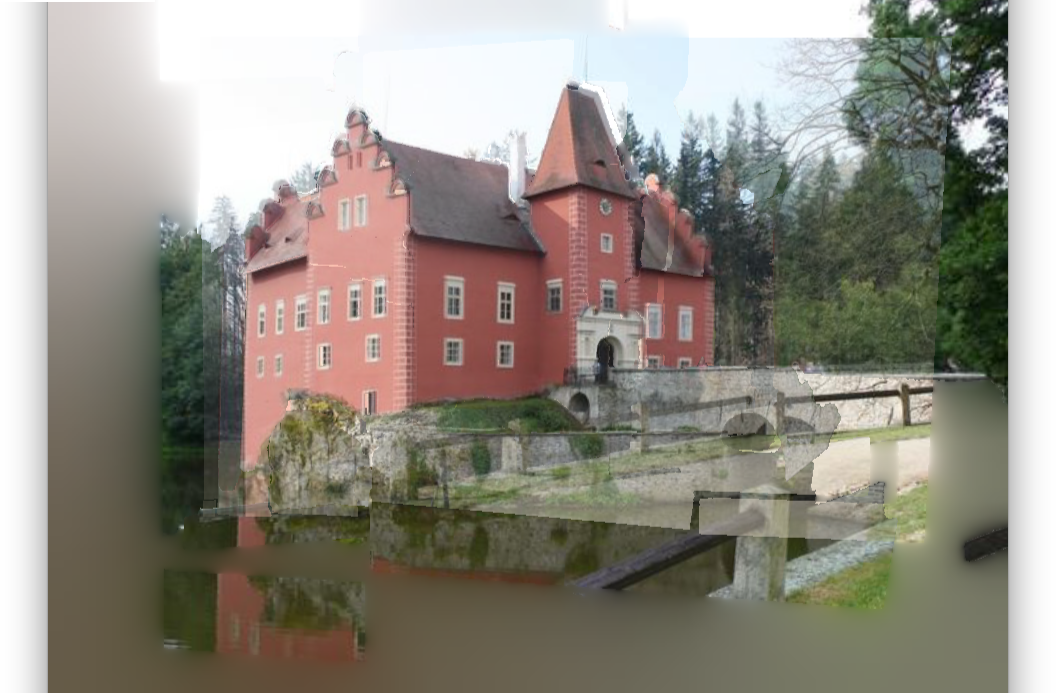
\includegraphics[keepaspectratio,width=\textwidth]{fig/Photosynth.png}
	\end{center}
	\caption{The Photosynth output of the Červená Lhota Castle in transition between several morphed images.}
	\label{fig:visualsfm}
\end{figure}

\subsection*{VisualSFM}
The Chungchang Wu's Visual Structure from Motion System is a GUI application for 3D reconstruction using structure from motion (SFM). The reconstruction system is modular and integrates several of other projects: SIFT on GPU(SiftGPU), Multicore Bundle Adjustment, and Towards Linear-time Incremental Structure from Motion. VisualSFM runs fast by exploiting multicore parallelism for feature detection, feature matching, and bundle adjustment. For dense reconstruction, the program supports Yasutaka Furukawa's PMVS/CMVS tool chain, and can prepare data for Michal Jancosek's CMP-MVS. In addition, the output of VisualSFM is natively supported by Mathias Rothermel and Konrad Wenzel's SURE.

The software follows the overall 3D reconstruction pipeline; It detects features using SIFT detector and SIFT extractor, matches feature pairs with the N-View Match, estimates the camera model for each image, removes images' distortion and then runs the dense reconstruction. Outputs of feature extraction and matching are stored as a binary files and are loaded if provided to save processing time. This enables use of other than built-in extractors and matcher, at least for the sparse reconstruction. \cite{www:visual_sfm}

\begin{figure}[ht]
	\begin{center}
		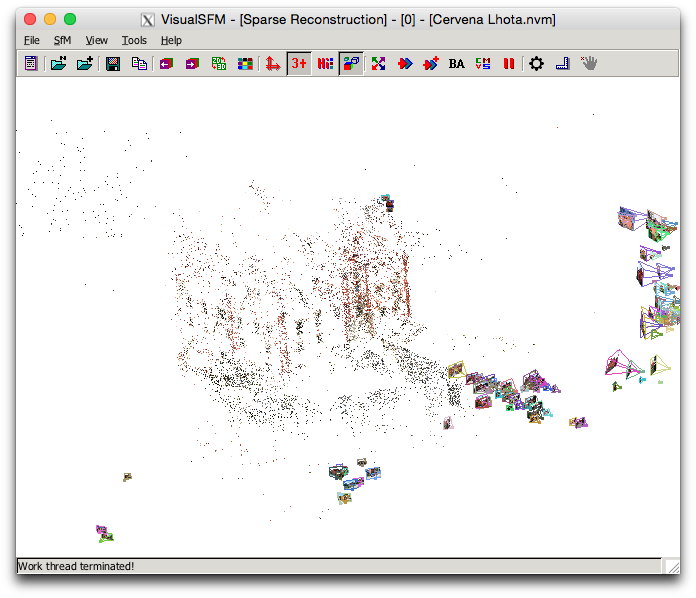
\includegraphics[keepaspectratio,width=\textwidth]{fig/VisualSFM.png}
	\end{center}
	\caption{The VisualSFM application GUI with sparse reconstruction of the Červená Lhota Castle.}
	\label{fig:visualsfm}
\end{figure}

\subsection*{Bundler}
Bundler is first well known Structure from Motion (SfM) system for unordered image collections from Noah Snavely. One of the first version of this Bundler system was used in the Photo Tourism project that was aqired by Microsoft and is now part of Photosynth. 

As other applications discussed, Bundler takes a set of images, image features, and image matches as input, and produces a 3D reconstruction of camera and sparse scene geometry as output. In order to get sparse point clouds, one has to run Bundler to get camera parameters, use the Bundle2PMVS program to convert the results into PMVS2 input and then run PMVS2. The system reconstructs the scene incrementally, a few images at a time, using a modified version of the Sparse Bundle Adjustment package of Lourakis and Argyros as the underlying optimization engine. Bundler has been successfully run on many Internet photo collections, as well as more structured collections. \cite{www:bundler}

\section{Detectors}
\label{sec:detectors}
A successful 3D reconstruction stands and falls on good features detection.The quality and robustness of features is (usually) much more important then their quantity which will be demonstrated by the Dense detector later in this section. The ideal feature detector finds salient image regions such that they are repeatedly detected despite change of viewpoint; more generally it is robust to all possible image transformations. Therefore, it does not detect any points in uniform and uninteresting surfaces like sky or texture-less walls. The best detector to be used depends heavily on the requested task. In our application features we are interested in are edges and corners of buildings and their distinct parts.

We can divide types of image features into following categories (please note that a detector can detect features from multiple categories):
% CITATION NEEDED!!!
\begin{itemize}
	\item \textbf{Edge} is a point where there is a sudden change between adjacent pixels (strong gradient magnitude). Generally an edge can be of almost any arbitrary shape and may include junctions. Locally edges have a one-dimensional structure.
	\item \textbf{Interest point} has a local two dimensional structure. We can think of it as two-dimensional edge, in fact early algorithms were used to detect interest points as edges and then selected the interest points by further calculation. In some literature you the interest points may be referred to as corners.
	\item \textbf{Blobs} provide a complementary description of image structures in terms of regions, as opposed to corners that are more point-like. A term regions of interest or interest points are sometimes used as the blob descriptors often contain a preferred point (a local maximum or a center of gravity). Blobs allows detection of smooth areas in an image that might not be detected as an edge or corner.
	\item \textbf{Ridges} are in computer vision a set of curves whose points are have a local maximum in at least one dimension. This notion captures the intuition of geographical ridges. Ridge detection is usually much harder then Edge, Interest point or Blob detection.
\end{itemize}

In the remainder of this section feature detectors implemented in the SLAM++ frontend using OpenCV will be presented. Each detector will be run on the same set of images with historic landmarks in order to evaluate the effectiveness and speed. Then a summary of the results will be presented.
 
\begin{itemize}
	\item The \textbf{Robust Invariant Scalable Keypoints (BRISK)} detector uses scale-space pyramid layers of octaves and intra-octaves to detect corners in an image. The algorithm uses FAST feature detector score and was developed to get the better of SIFT and SURF detectors. However, in our case the performance gain is not worth decreased feature quality. \cite{article:brisk}
	
	\item \textbf{Dense Sampling} uses a regular grid to find a keypoints in the image. This results in good coverage of the entire object or scene and a constant amount of feature per image area. The dense sampling is fast as the detector selects all points on a grid without analysis of the surrounding. On the downside, dense sampling cannot reach the same level of repeatability as obtained with interest points, unless sampling is performed extremely densely, but then the number of features quickly grows unacceptably large. The dense sampling is therefore not useful in the SfM model estimation, but can be used for a dense reconstruction once sparse structure is calculated. \cite{article:dense}
	
	\item The \textbf{Features from Accelerated Segment Test (FAST)} aims to rapidly increase performance of feature detection while sustaining feature quality of SIFT-like detectors. The algorithm detects corners in the image and should be used with SIFT or SURF extractor for best performance. As the FAST select in our case three times more features hundred times faster than SIFT (resp. 50 times faster than SURF) we market this as one of the interesting detectors for the final implementation. \cite{article:fast}
	
	\item One of the most known feature detectors is the \textbf{Harris Corner Detector} . It can identify similar regions between images that are related through affine transformations and have different illuminations. Even though the Harris Corner Detector is fast, it does not select enough keypoints and therefore is not suitable for the 3D building reconstruction. \cite{www:harris}
	
	\item The \textbf{Good Features to Track (GFTT)} detector is modified version of the Harris Corner Detector described earlier. It is still classified as a corner detector, however, the scoring function differs. Compared to the Harris, the algorithm was slightly slower, with higher amount of features. Nevertheless, both of these algorithms do not perform well enough for our problem. \cite{article:gftt}
	
	\item The \textbf{Oriented FAST and Rotated BRIEF (ORB)} detector originated from the OpenCV Labs. It's goal was to offer robustness of a SIFT and SURF, while maintaining fast processing time like FAST and BRIEF combination. While this may be true, for our problem the ORB detector does not perform well enough. The feature found rarely belong to a building and usually chunks around trees and vegetation. \cite{www:orb}\cite{article:orb}
	
	\item The \textbf{Maximally Stable Extremal Regions} is a blob detector. For our task this detector performs poorly and takes even more time than SIFT detector.
	
	\item A \textbf{Scale Invariant Feature Transform (SIFT)} keypoint is image region with an orientation. The detector uses as a keypoints image structures  which resemble blobs. The use of the detector is licenced which is one of the reasons why we would like to use a different detecter. However, as expected, the detector performs very well and is used by other SfM software we discussed earlier. \cite{article:sift}
	
	\item The \textbf{Speeded Up Robust Features (SURF)} detector is modification of the SIFT detector. It addresses slow processing of the SIFT while maintaining reasonable efficiency. While it can surely be used in the SfM application, from our experiments we discovered that the increased performance greatly decreases feature detection for (in our case) important structures.  \cite{www:surf}
\end{itemize}

We've implemented all of the standard OpenCV keypoints detectors from previous list in the SLAM++ frontend. The goal was to test how do they perform on our specific problem: detecting keypoints in buildings. The figure \ref{fig:detectors} shows three detectors (SIFT, SURF and FAST) that are suitable for our task as they find enough relevant features in an image. 

\begin{figure}[ht]
	\begin{center}
		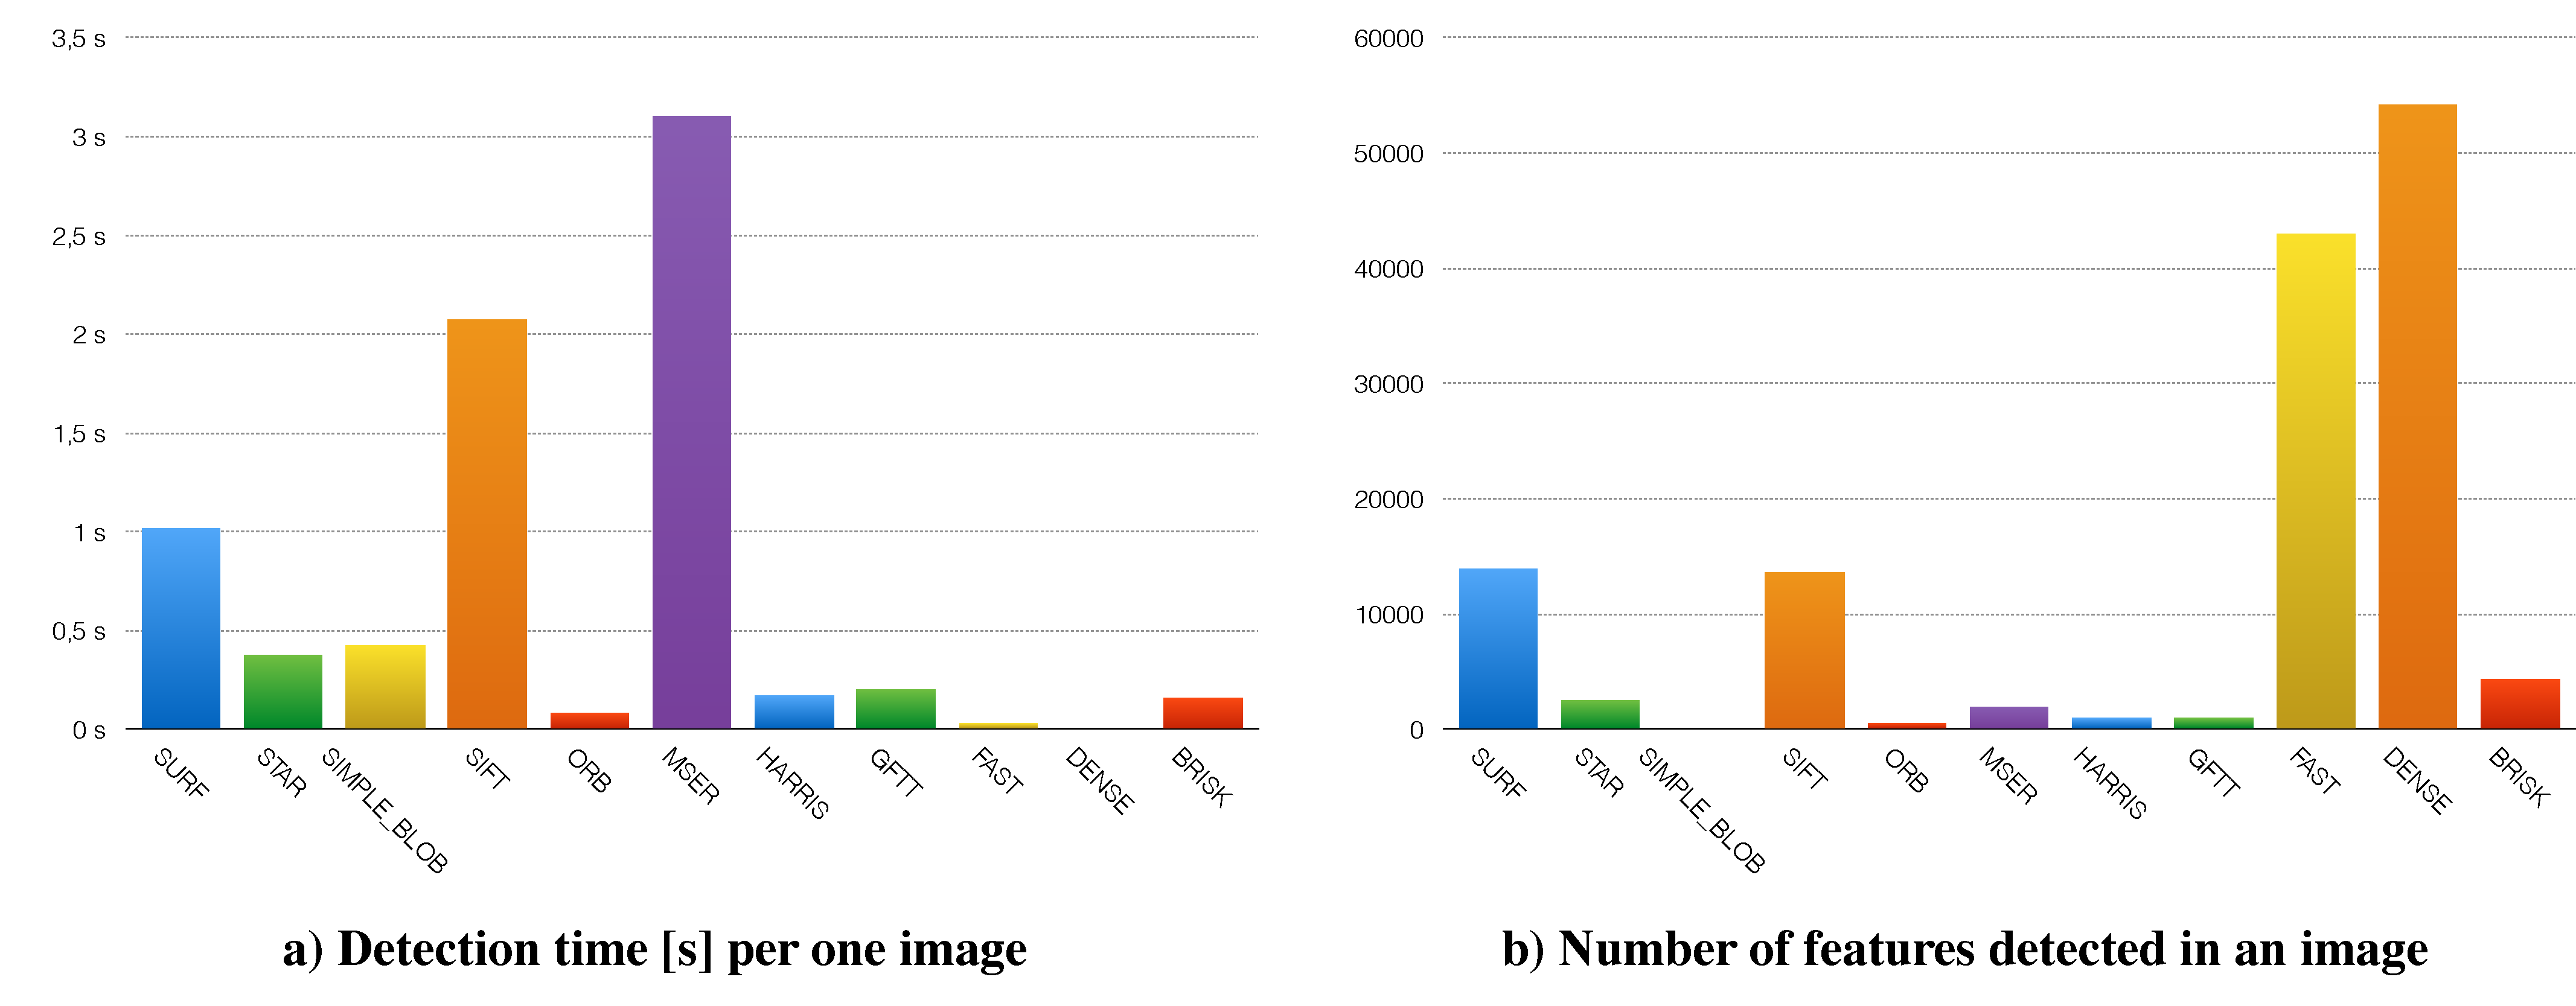
\includegraphics[keepaspectratio,width=\textwidth]{fig/detectors.pdf}
	\end{center}
	\caption{Results of the feature detection evaluation on as set of 500 various images from the Červená Lhota dataset. Graph a) shows average time necessary for processing an image using selected detector. In graph b) you can find how many features on average were detected in a single image.}
	\label{fig:detectors}
\end{figure}

\section{Extractors}
\label{sec:extractors}
In order to work further with the keypoints detected in previous step, the keypoints have to be analysed and transformed into so called feature descriptor. The process consist of inspecting local image patch around the keypoint to be extracted. This extraction may involve quite considerable amounts of image processing and involves reducing the amount of resources required to describe the original data. The result is known as a feature descriptor or a feature vector. Among the information that may be stored within feature descriptor, one can mention local histograms. In addition to such attribute information, the keypoints detection step may also provide complementary attributes, such as the edge orientation, gradient magnitude in edge detection and the polarity or the strength of the blob in blob detection. The authors of detectors usually specify which extractor should work best for their detection algorithm, some even provide their own. Nevertheless, we tried all combinations with detectors to get the best results for our application.

There are two types of descriptors in the OpenCV that are now available in Slam++ frontend; a) descriptors using floating point and b) descriptors storing information as a binary data in unsigned char type.
\begin{itemize}
	\item[a)] \textbf{Float} descriptors:
	
	\begin{itemize}
		\item \textbf{SIFT:} The scale-invariant feature transform of a neighbourhood is a 128-dimensional vector of histograms of image gradients. The region, at the appropriate scale and orientation, is divided into a $4\times 4$ square grid, each cell of which yields a histogram with 8 orientation bins. The SIFT extractor is advised to be used with the SIFT, SURF and FAST detector.
		\item \textbf{SURF:} The speeded up robust feature extractor uses either 128 or 64-dimensional vector of histograms of image gradients.An oriented quadratic grid of $4 \times 4$ square sub-regions is laid over the keypoint and a wavelet response computed for each square. According to literature the SIFT, SURF and FAST detector can be used with the SURF extractor. \cite{www:sift_surf}
	\end{itemize}
	
	\item[b)] \textbf{Binary} descriptors:
	
	\begin{itemize}
		\item \textbf{BRIEF:} The Binary Robust Independent Elementary Feature descriptor is a 128, 256 or 512-dimensional bitstring which is a good compromise between speed, storage efficiency and recognition rate. The descriptor is much smaller (16, 32 or 64 bytes) compared to floating point descriptors, while maintaining a good performance compared to SURF or U-SURF. \cite{article:brief}
		
		\item \textbf{ORB:} Unlike BRIEF, Oriented FAST and Rotated BRIEF (ORB) is comparatively scale and rotation invariant while still employing the very efficient Hamming distance metric for matching. As such, it is preferred for real-time applications, but may be suitable for some offline applications as well. \cite{www:orb}\cite{article:orb}
		
		\item \textbf{FREAK:} The Fast Retina Keypoint extractor aims to be faster and more robust than SIFT and SURF. It uses a novel keypoint descriptor inspired by the human visual system to compute cascade of binary strings.\cite{article:freak}
		
		\item \textbf{BRISK:}  The  Binary Robust Invariant Scalable Keypoints extractor uses a 64-byte binary descriptor composed as a binary string by concatenating the results of simple brightness comparison tests. \cite{article:brisk}
	\end{itemize}
\end{itemize}

\section{Matchers}
\label{sec:matchers}
So far we are able to find points of interest in an image and describe them in such a way that they are effectively stored but still contain information about the point and its local image patch. Once descriptors are extracted from two or more images, we want to match points that are visible in more then one image. This is called nearest neighbour search which is an optimization problem for finding closest (or most similar) points. There are two approaches to this problem that are implemented in the OpenCV: Brute-Force and FLANN-based matching.

The Brute-Force matcher is simple and naive approach. It takes the descriptor of one feature from the first image set and matches it with all other feature from the second image set. During the process a distance of some sort is calculated and the match with best metric selected. There are number of metrics implemented in the OpenCV to be used with different descriptors, but we once again tried all the combination in order to get best result for our problem. The algorithm promises best possible matches, but due to the fact that it tries to match each pair of feature, can take a lot of time to process. 

The Fast Library for Approximate Nearest Neighbors (FLANN) implementad in OpenCV, performs a fast approximate nearest neighbor searches in high dimensional spaces. It uses the Hierachical K-means Tree for generic feature matching. Nearest neighbors are discovered by choosing to examine the branch-not-taken nodes along the way.

\begin{figure}[ht]
	\begin{center}
		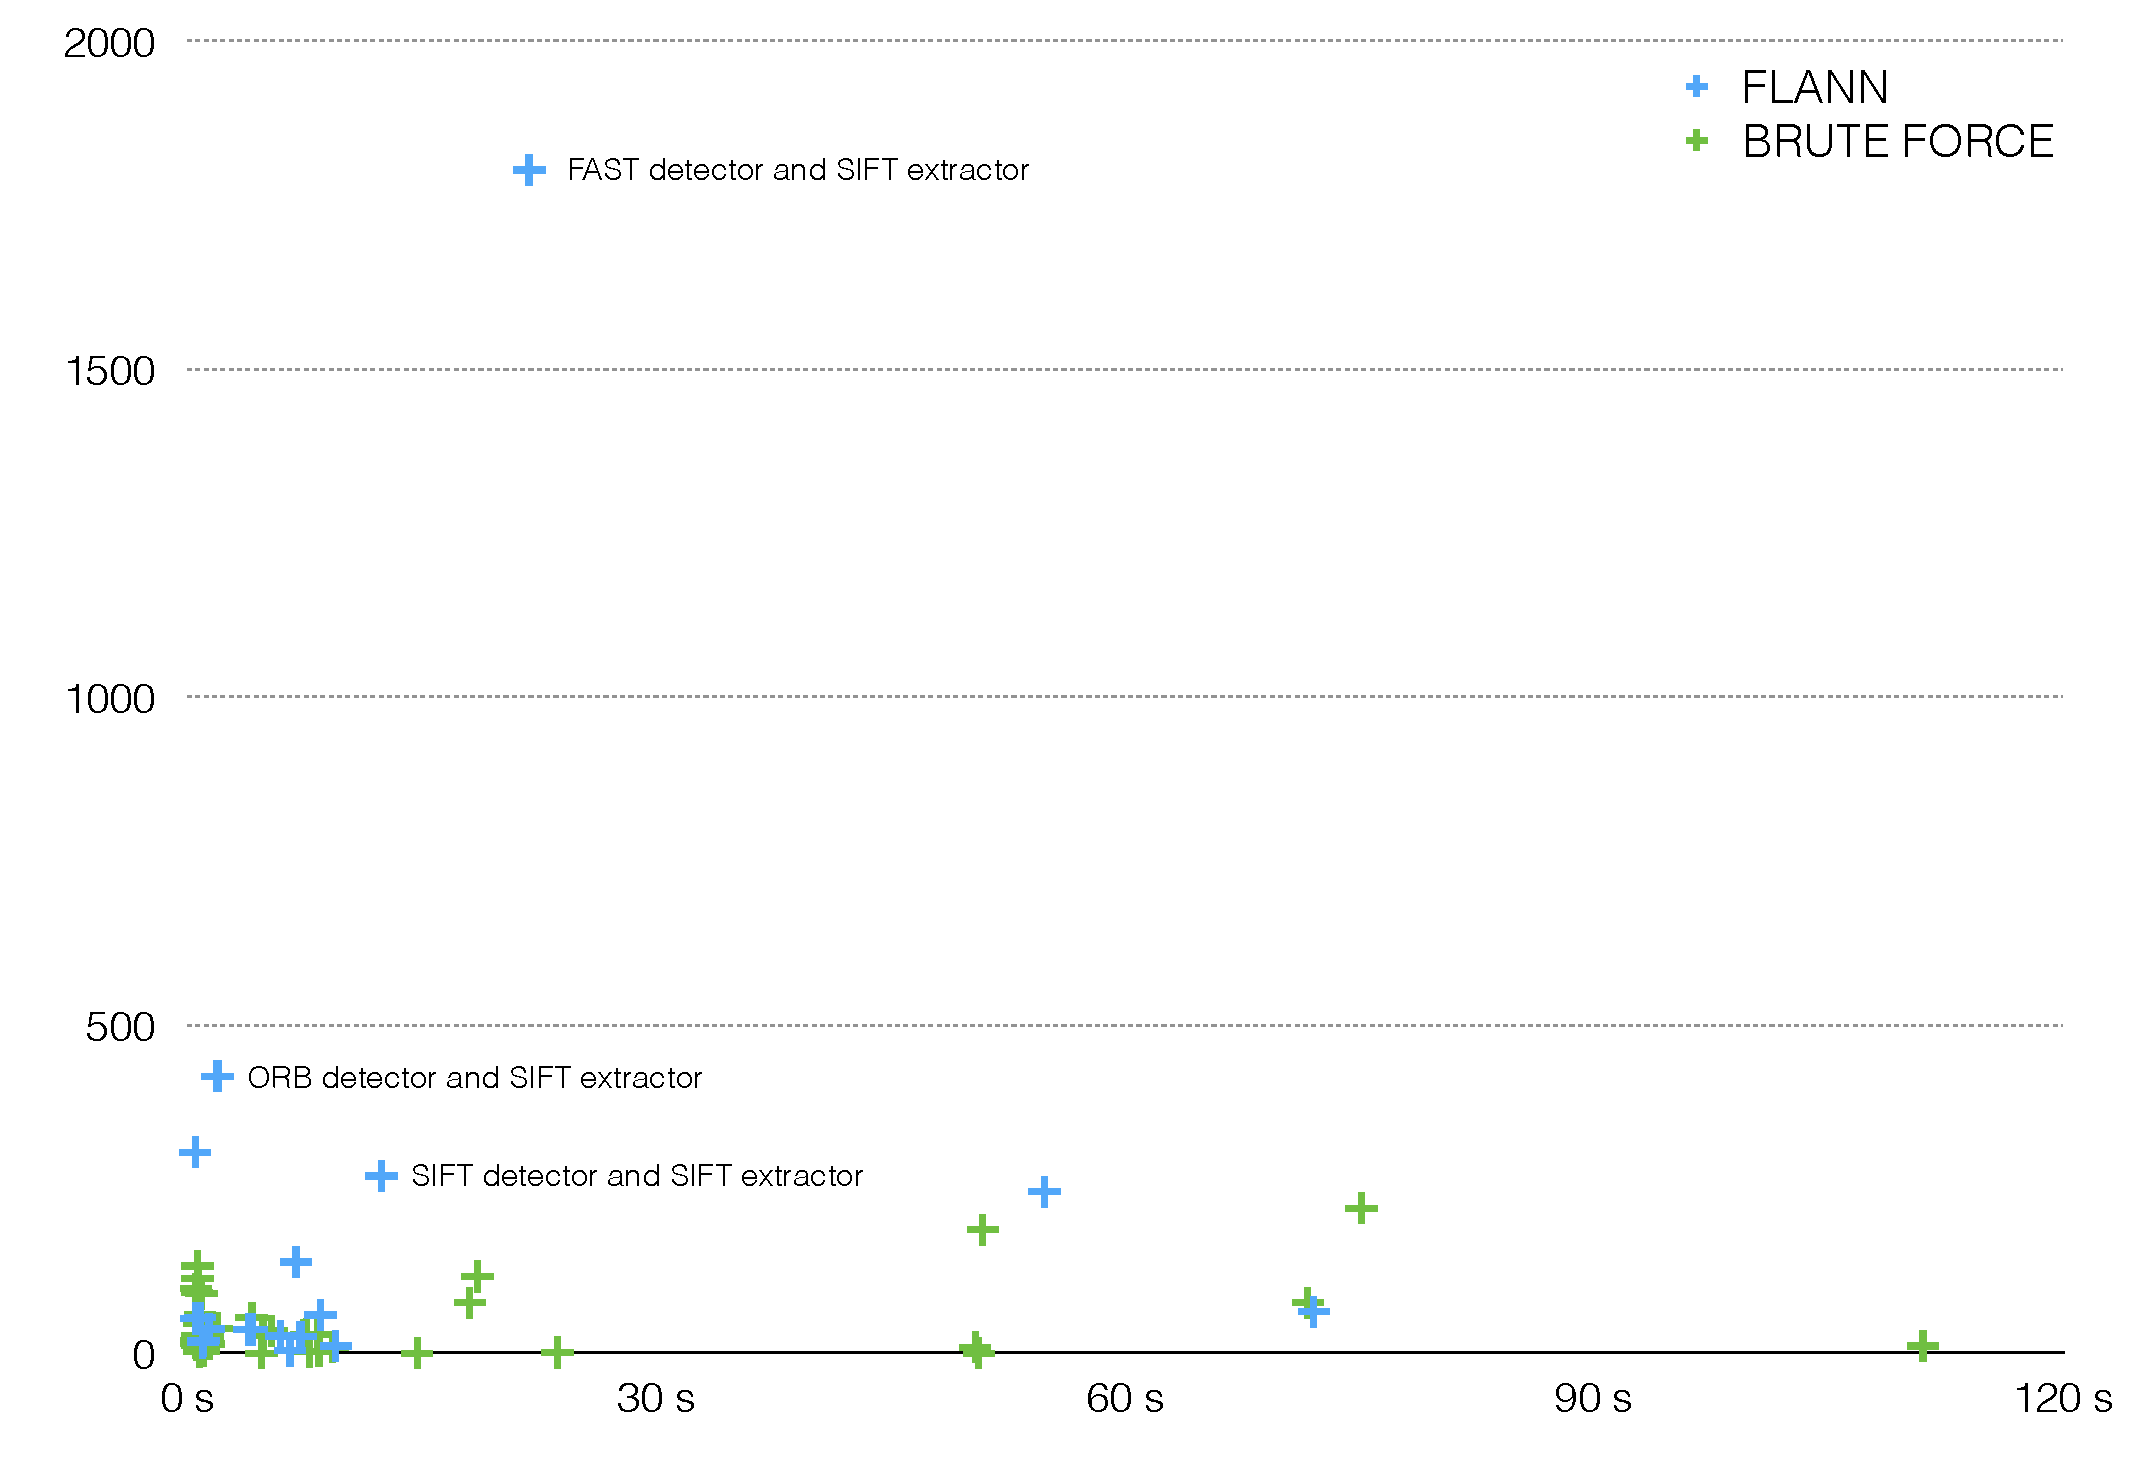
\includegraphics[keepaspectratio,width=12cm]{fig/matchers.pdf}
	\end{center}
	\caption{Results of the feature detection, extraction and matching evaluation on a set of 100 image pairs from the Červená Lhota dataset. The interesting combinations are labeled. Note that combination taking more than 120 seconds to compute were omitted.}
	\label{fig:matchers}
\end{figure}

We manually selected 100 image pairs from the Červená Lhota dataset and tried every feature detection, extraction and matching combination described in this chapter. The results are shown in figure \ref{fig:matchers}. To select only potentially good matches ($G$), following metric was applied

\begin{equation}
	0.02 \leq G \leq 2* M
\end{equation}

\ where $M$ is a minimal distance found between a match pair for selected images. From the results, we can conclude that best result, in terms of performance to effectiveness ratio, is achieved using FAST detector, SIFT extractor and FLANN matcher. The figure \ref{fig:matches} shows matches for one image pair using some of the well known feature detector, extractor and matcher combinations. The picture a) shows that the ORB detector is fast, but for our application does not yeld good results. The SIFT detector and extractor performs well and can be used for the SfM application. In fact it is being used by the VisualSfM program introduced earlier. The best obtained result is depicted in c) where FAST detector and SIFT extractor were used.

\begin{figure}[ht]
	\begin{center}
		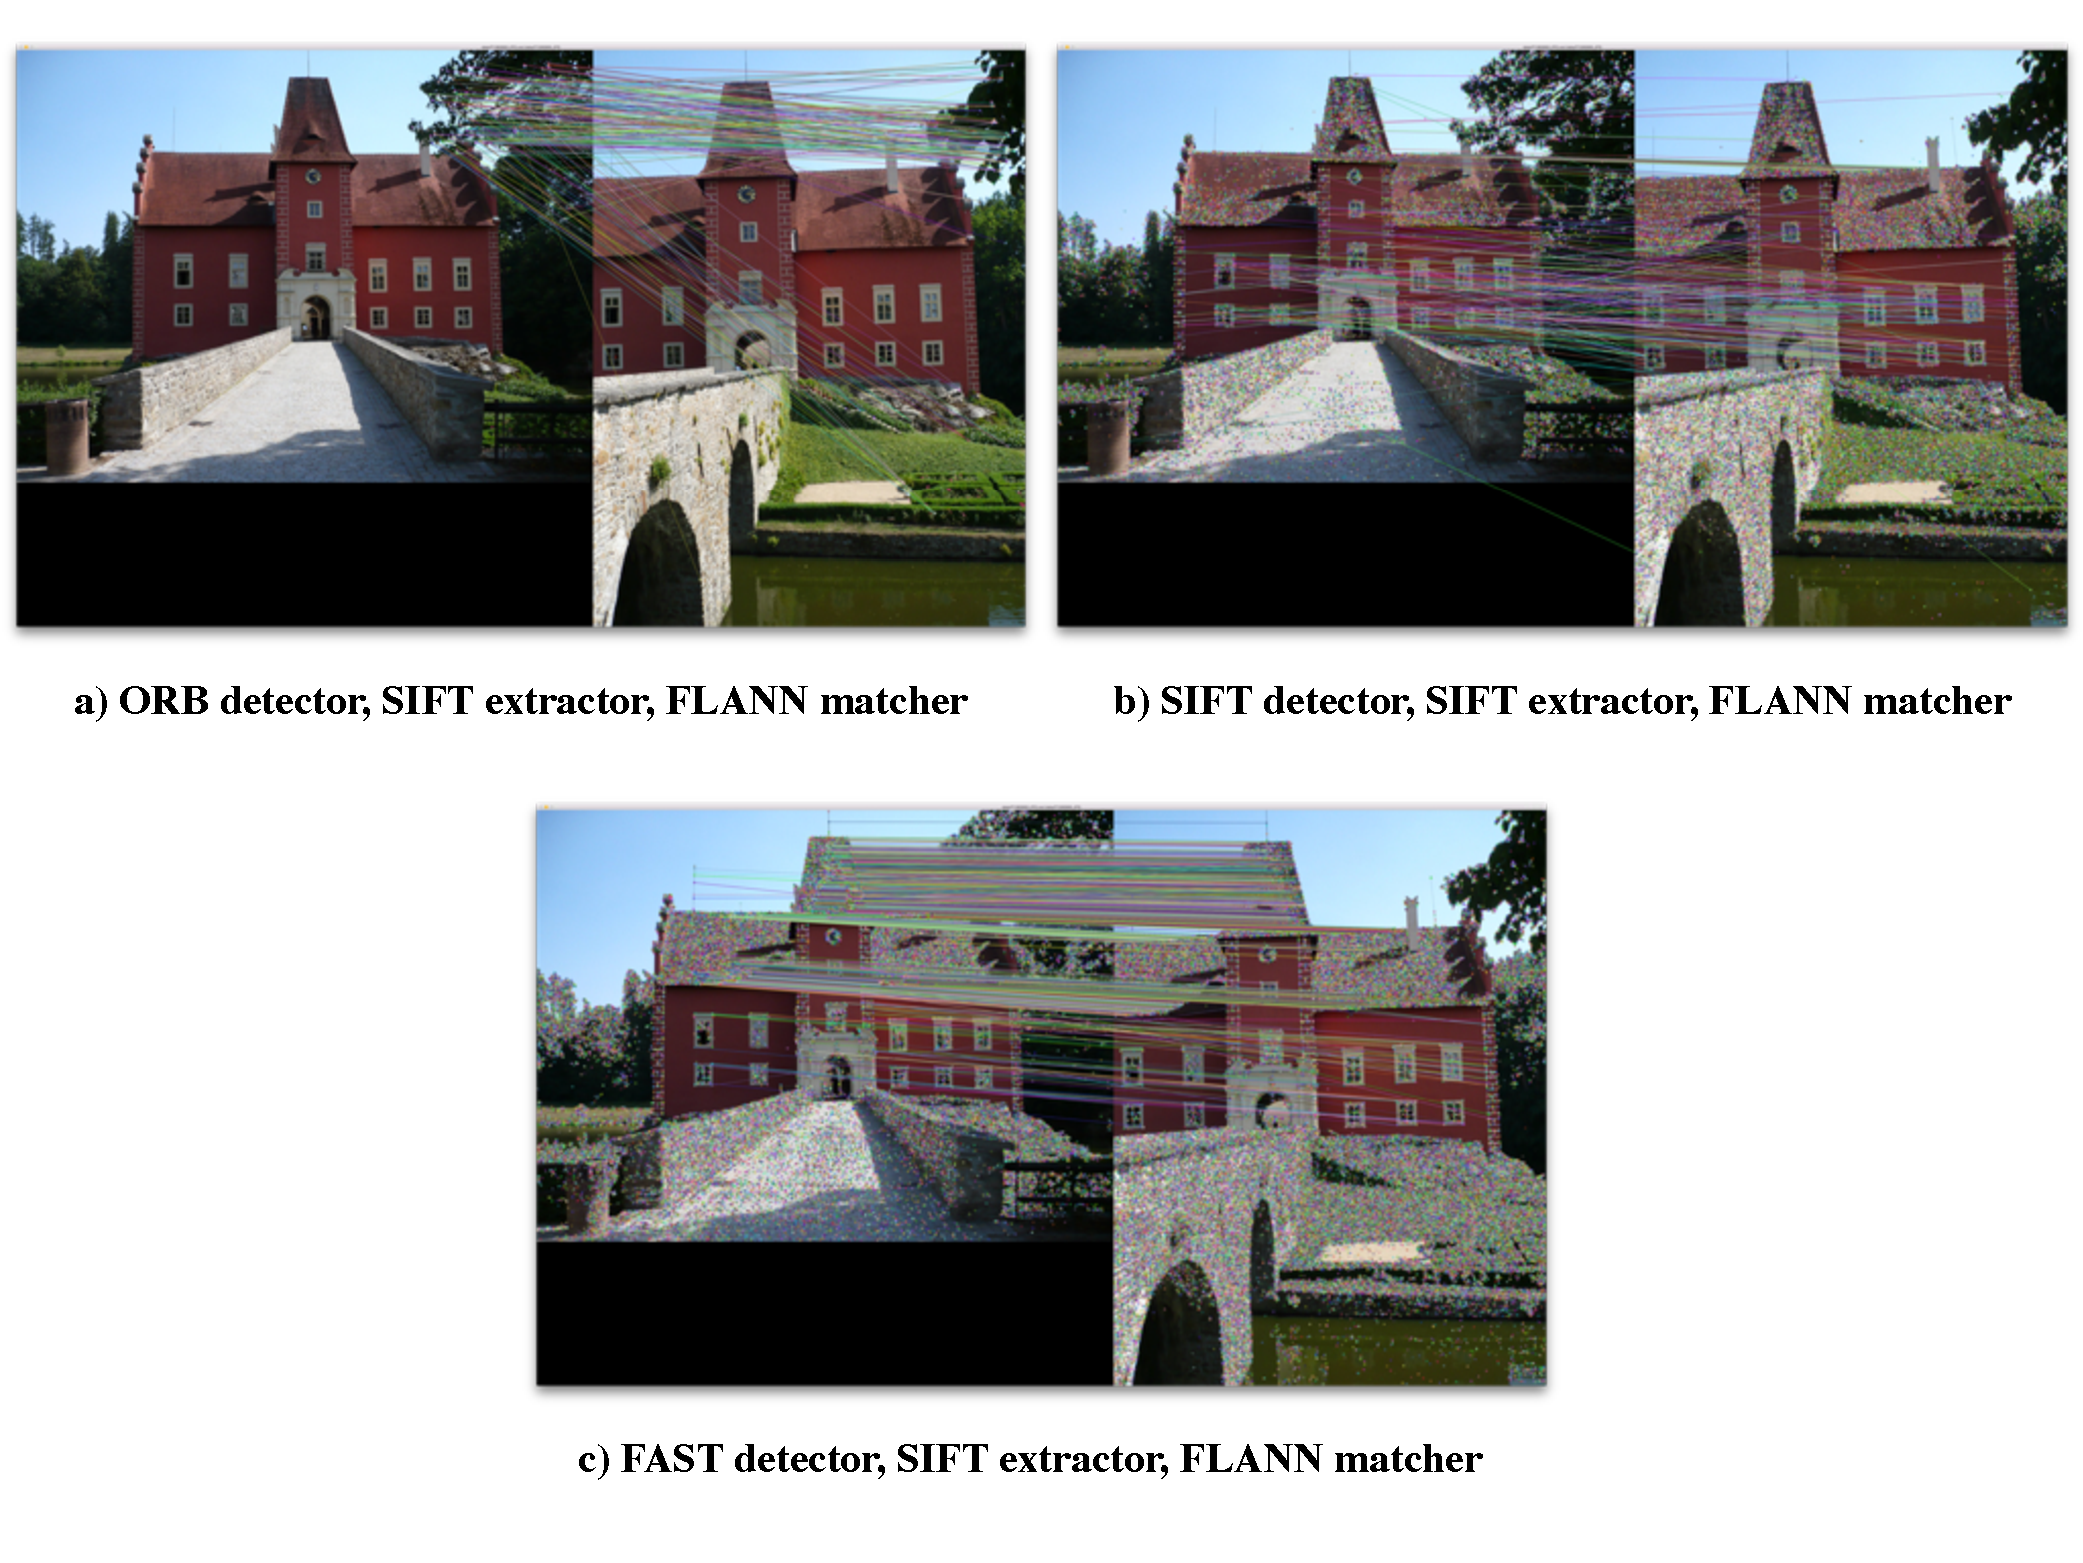
\includegraphics[keepaspectratio,width=\textwidth]{fig/matches.pdf}
	\end{center}
	\caption{Examples of various feature detector, extractor and matchers combinations on an image pair. There are 307 good matches in picture a) and the whole process took 0,487 seconds. The picture b) took 12.7 seconds to process and has 274 good matches. The last picture c) contains 1804 good matches and was processed in 23.853 seconds.}
	\label{fig:matches}
\end{figure}

\chapter{Methodology}
\label{chapter:methodology}
This chapter thoroughly describes the so far implemented part of the process of 3D reconstruction from a set of images. Steps that are not yet implemented are outlined and briefly discussed. The reader will be introduced to the dataset aquisition from the internet especially Flickr. Then the implemented feature detection, extraction and matching in context of 3D reconstruction. The next section discusses the 3D reconstruction approaches leading to the uncalibrated one which will be implemented. Finally we introduce the SLAM++ framework and it's application in this project. 

\section{Three-dimensional Structure Estimation Pipeline}
The pipeline (depicted in figure \ref{fig:pipeline}) for the implemented solution is similar to the pipeline described in section \ref{sec:existing_3D_reconstruction_solutions}. Firstly we create a dataset by downloading images from the internet. These images are then filtered and used as an input for the implemented application called uncalibrated app. The uncalibrated app detects and extracts features from the input image set and finds the matches between every image. As of now these are the steps implemented. Next steps, which will be soon implemented, includes the camera initialization and pose estimation. Finally this allows us to calculate the model's 3D structure from the points seen by different cameras. As of now there are no plans to implement visualization of a final sparse reconstruction, but the SLAM++ fremework provides a means to visualize the resulting sparse point cloud. 

\begin{figure}[ht]
	\begin{center}
		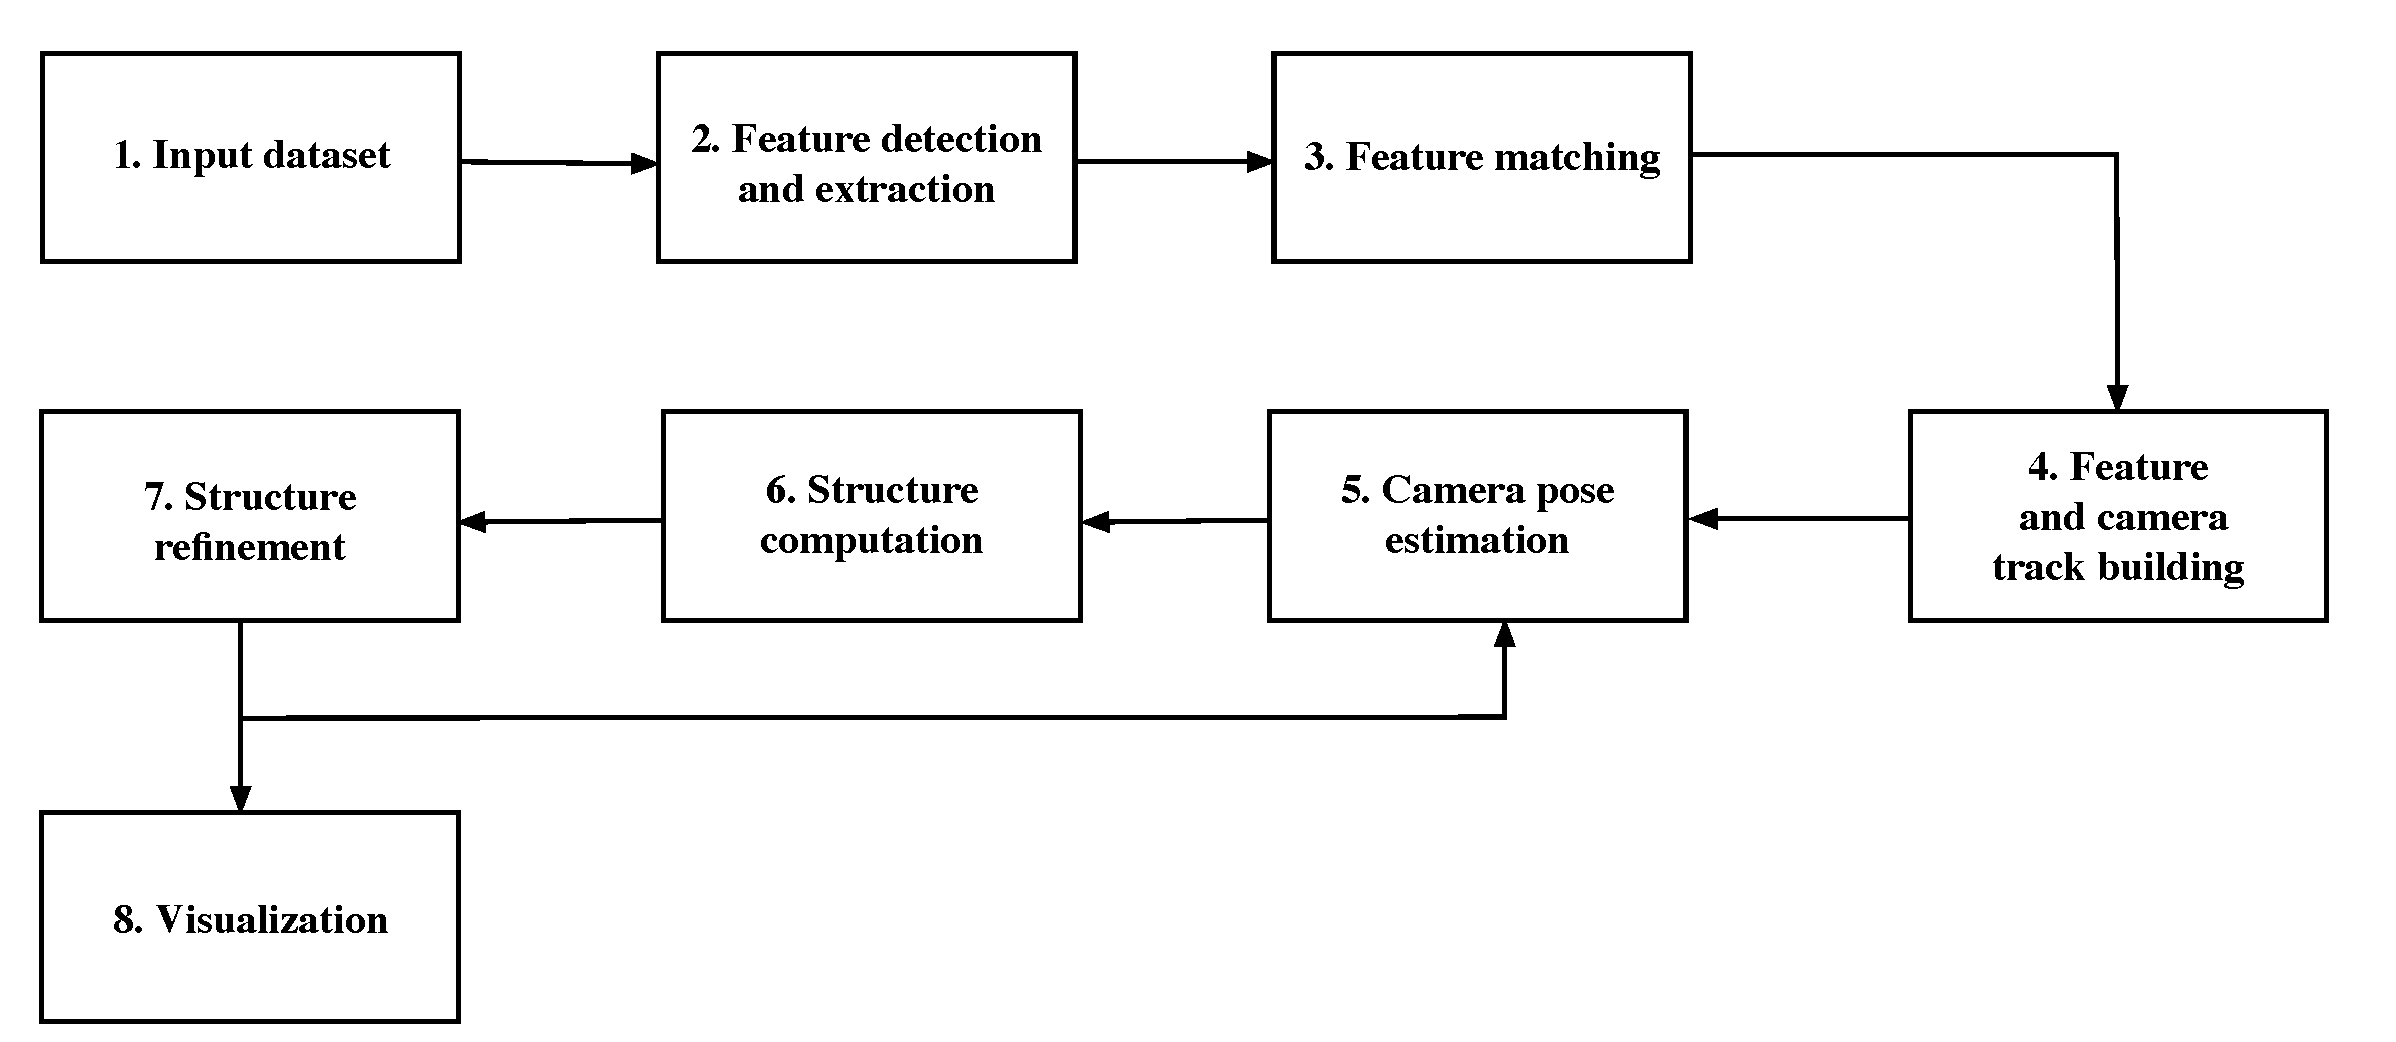
\includegraphics[keepaspectratio,width=\textwidth]{fig/pipeline.pdf}
	\end{center}
	\caption{The three-dimensional structure from two-dimensional images estimation pipeline.}
	\label{fig:pipeline}
\end{figure}

\subsection*{Dataset Generation}
Creating a dataset is a crucial part of the process of estimating three-dimensional structures from two-dimensional image sequences. The dataset has to contain enough images with a feature pairs to be vialable for reconstruction. We also want to filter out images taken during the night or throughout various seasons as the depicted object and its surroundings may change significantly.

With this in mind we've decided to download images from Flickr webpage. Flickr is well known and widely used web service for sharing pictures. The advantage of this service, in comparison to other picture sharing websites, is the ability to tag the photo. Each image can contain a number of tags describing the photo. Most of the pictures uploaded contain information about the place where the photo was taken and can be aggregated using such this tag. A tool, Flickr downloader, we designed allows downloading images from Flickr in batches based on the tag. It is a simple Python script taking two parameters; number of photos to be downloaded and a tag of the image. The script connects to the Flickr webpage, downloads the search results page, cyclically opens each photo page and downloads the image. The downloaded images are stored to the \texttt{downloaded} output folder.

While the Flickr yelds good results for well known places in countries like USA or western Europe, there is not enough images in the Czech Republic yet. This is the reason why we have, for now, decided to use different services, like Google image search, as well. The datasets aquired were manually filtered to eliminate irrelevant images and limit the selection to daytime photos taken in summer.

\subsection*{Feature Detection, Extraction and Matching}
Once we have a desired dataset we compute the feature pairs. An interface between the SLAM++ and the OpenCV was created which allowed use of the feature detectors, extractors and matchers described in chapter \ref{chapter:the-state-of-the-art}. The interface is a C++ template so there is no overhead. The extractors are defined using the \texttt{typedef} keyword and naming convention follows this scheme: \texttt{FeatureExtractor\_OpenCV\_[detector]\_[extractor]}.

In the building reconstruction the repeated features are common. Many objects, such as clock towers with nearly identical sides, or domes with strong radial symmetries, pose challenges for structure from motion. When similar but distinct features are mistakenly equated, the resulting 3D reconstructions can have errors ranging from phantom walls and superimposed structures to a complete failure to reconstruct. This can be partially solved by a good selection of the feature detecting, extracting and matching algorithms. In section \ref{sec:matchers} we have identified some combinations that yeld good feature matches and therefore are suitable for the Structure from Motion algorithms on building reconstruction. We will use these algorithms int the uncalibrated app once it is finished.

\section{3D Reconstruction Approaches}
Based on the image source we can distinguish between three types of vision: Stereoscopic, Monocular and Uncalibrated. The type of the vision defines the difficulty of the 3D reconstruction problem.

\subsection*{Stereoscopic Vision}
The stereoscopic vision is similar to human binocular vision. Two cameras, displaced horizontally from one another are used to obtain view of the scene, simulating human vision. By comparing both images, the relative depth information can be obtained, which is proportional to the differences in distance to the objects. If the images are undistorted, and camera parameters known, we can easily calculate the 3D relative position of the points. The figure \ref{fig:stereo} shows how the depth can be calculated using following equation:

\begin{equation}
	z=\frac{f b}{x_L - x_R}
\end{equation}

If the cameras are calibrated then the reconstruction is straightforward as the depth is the only thing required to calculate the position in the 3D image.

\begin{figure}[ht]
	\begin{center}
		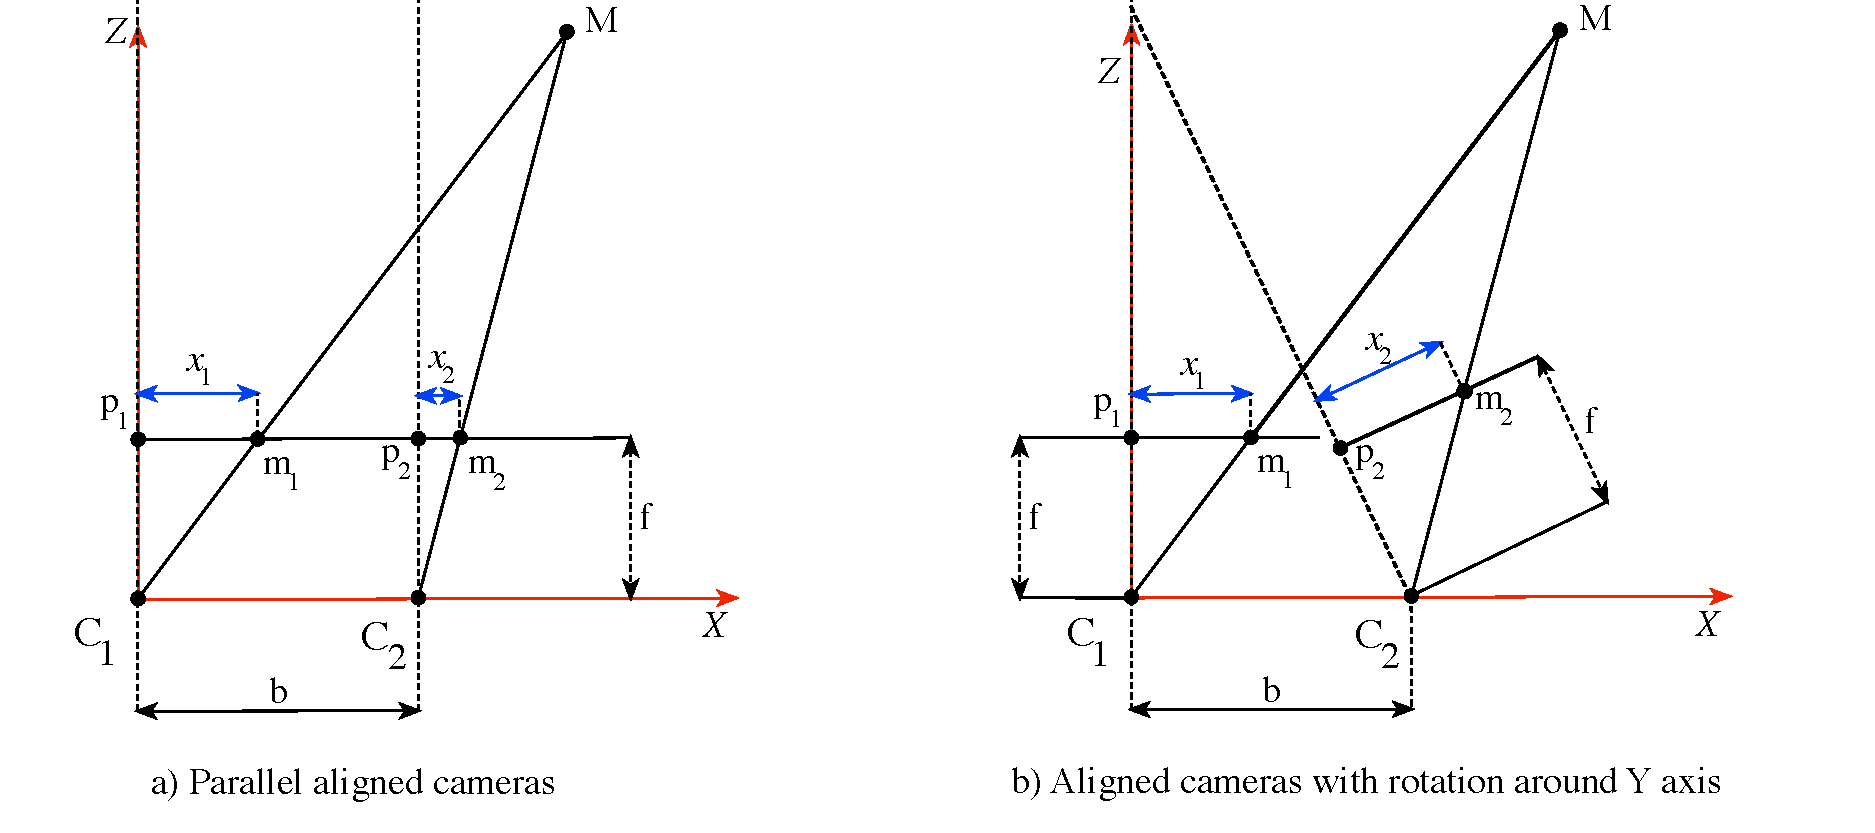
\includegraphics[keepaspectratio,width=9cm]{fig/stereo.pdf}
	\end{center}
	\caption{An illustration of obtaining the depth information from stereo image.}
	\label{fig:stereo}
\end{figure}

\subsection*{Monocular Vision}
The monocular vision consists of one camera moving in space. Because we have only one camera, we can't easily calculate the depth as in stereoscopic vision, but we need to estimate the camera position first. Firstly we detect feature in images and match them. Now that we have paired points in images, we can begin to estimate the camera position. At least three image pairs are needed in order to calculate the camera pose, other points can increase the accuracy of the solution. Once camera position is known, the 3D structure can be calculated. However, because the picture is distorted and pixels have limited precision the structure will introduce some error. In order to minimize the reprojection error, we run a bundle adjustment algorithm.

\begin{figure}[ht]
	\begin{center}
		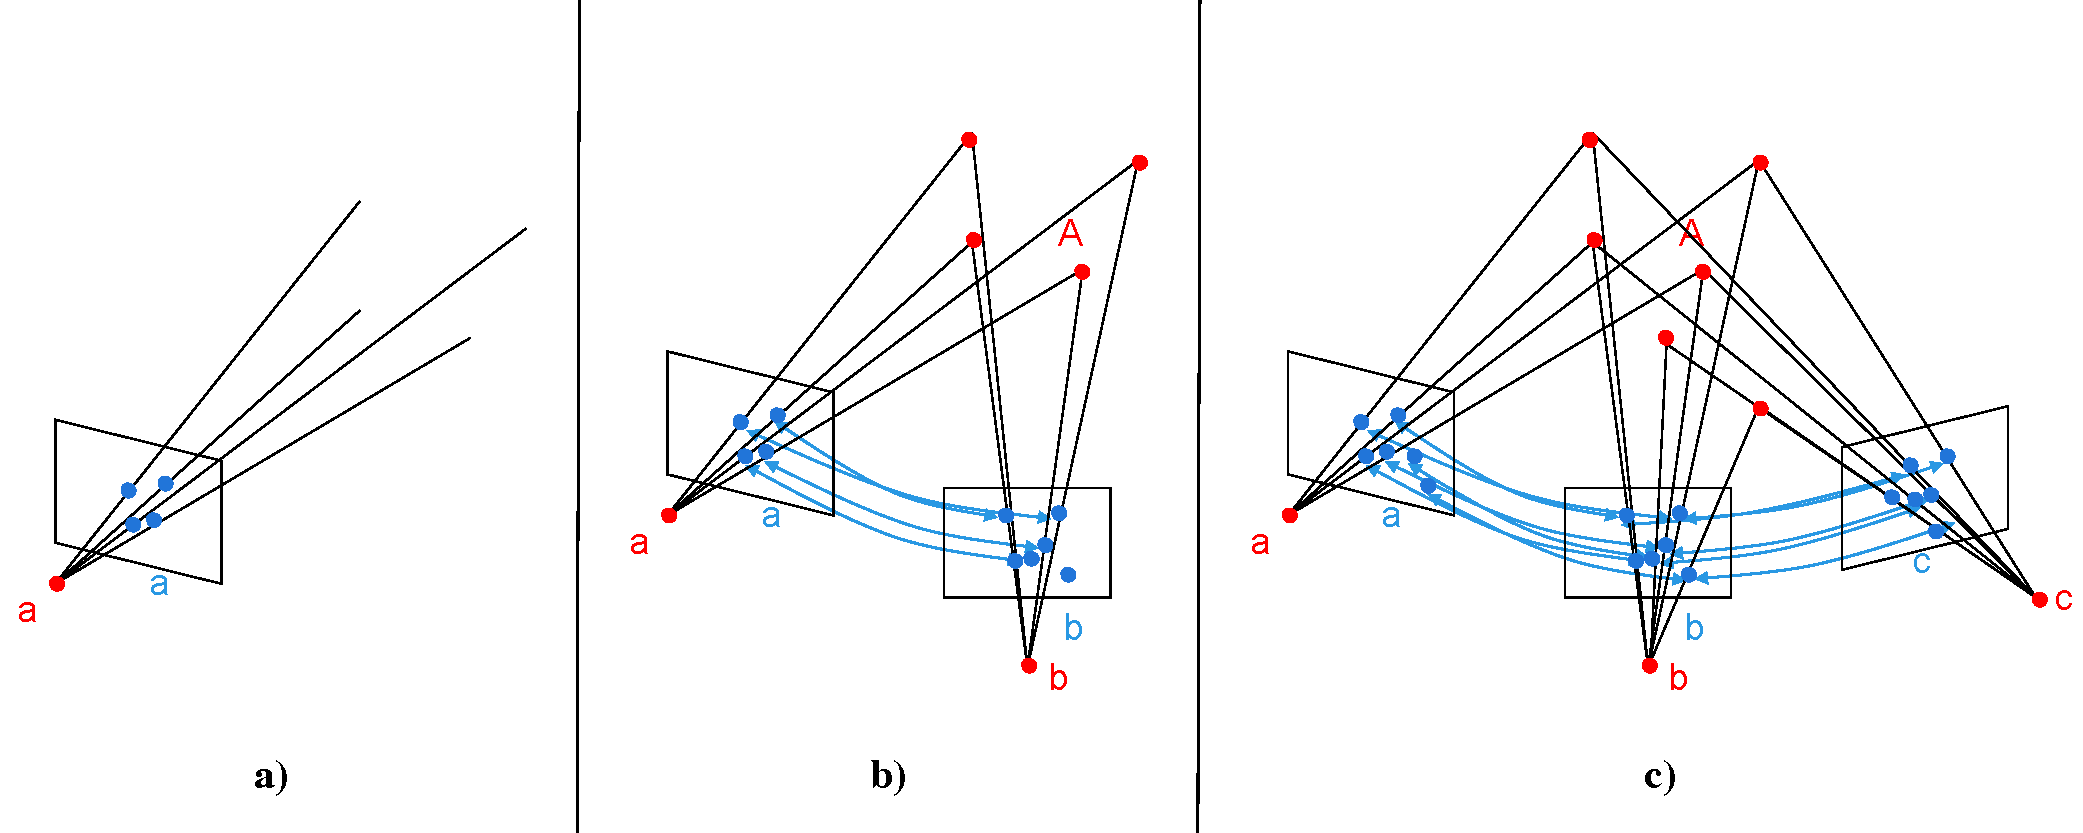
\includegraphics[keepaspectratio,width=\textwidth]{fig/mono.pdf}
	\end{center}
	\caption{An illustration of the process of 3D reconstruction using a monocular vision. a) detect features b) match them and estimate camera pose c) add other points with next iteration. This image was taken from the Monocular camera 3D reconstruction presentation by Ing. Marek Šolony.}
	\label{fig:stereo}
\end{figure}

\subsection*{Uncalibrated Vision}
Until this point the camera parameters were known or could have been easily estimated. However, when dealing with images downloaded from the internet, we don't have such information. This makes the problem much more complex and to find the solution we not only need to estimate camera position but also it's parameters. The principle of reconstruction is similar as in the monocular vision, but we need 8 points instead of 3 to calculate the two-dimension to three-dimension transformation. Once the camera calibration and position is known, we can undistort the images and calculate the 3D structure.

\section{SLAM++ Frontend and Backend}

\chapter{Conclusion and Further Work}
\label{chapter:conclusion}
This chapter presents the conclusion of the term project work. Next steps are also outlined as this topic will be further developed as a part of the Masters thesis.

\section{Conclusion}
This term project has focused on the study of a means to estimate three-dimensional information from a two-dimensional image sequence. Usually, the first step is to create appropriate dataset. We summarized requirements on such dataset, identified what qualities the images should have and what sort of images should be filtered out. We provided a simple tool that allows downloading images in batches from the Flickr service and explained why we have decided to use additional sources of images as well. 

Another step in the 3D reconstruction is detection of the feature. A number of feature detectors were introduced and their characteristics described. We conducted a series of experiments which goal was to understand qualities of feature detections in context of the building reconstruction. Then the reader was introduced to the issue of extraction of the feature descriptors from the image. The extractors implemented in OpenCV were described and compared one to another. We finished the chapter with feature matching algorithms. All combinations of feature detectors, extractors and matchers were tested on a 100 image pair input set and the result evaluated. We've selected the best combination, FAST detector, SIFT extractor and FLANN matcher, for our problem which maintains a good ratio between performance and efficiency.

The problem of 3D information estimation was discussed and three different approaches of non-contact scanning outlined. We started with the stereo vision, where the depth can be directly computed from the image disparity. The problem gets more difficult when only one camera scans the 3D space. This approach, monocular vision, uses feature to calculate camera position and reconstruct the 3D structure. Lastly we talked about the uncalibrated approach, where the scene is being reconstructed from a number images made by multiple cameras, each having a different calibration matrix. The pose estimation was outlined and difficulties with such approach identified.

Lastly we talked about existing solutions that are implementing the uncalibrated approach. Three different programs (Photosynth, VisualSFM and Bundler) were introduced and briefly evaluated. These programs will be matched against the final application implemented within the Masters thesis to evaluate its capabilities and performance.

\section{Further Work}
The research and work presented in this paper proposes the following subjects for further work:
\begin{itemize}
	\item Completion of the feature detection and matching part of the uncalibrated app. As of now, the program can detect and match feature, however, it would be useful to store such information in a binary form to be able to use it as a input for the VisualSFM. This would allow us to test how does the reconstruction improve with a different detector.
	
	\item A further steps should be implemented into the uncalibrated app. This includes camera calibration and pose estimation and the 3D structure reconstruction. The result of this step will be sparse point cloud that can be visualized using software like Meshlab.
	
	\item With the application being able to create sparse reconstruction, further description of the math behind the problem needs to be provided. This includes but is not limited to fundamental matrix estimation, camera calibration and epipolar geometry.
\end{itemize}
%=========================================================================
 % viz. obsah.tex

  % Pouzita literatura
  % ----------------------------------------------
\ifczech
  \bibliographystyle{czechiso}
\else 
  \bibliographystyle{plain}
%  \bibliographystyle{alpha}
\fi
  \begin{flushleft}
  \bibliography{literatura} % viz. literatura.bib
  \end{flushleft}
  \appendix
  
  \chapter{Contend of the DVD}
\begin{itemize}
	\item \textbf{thesis.pdf} - PDF version of the thesis text.
	\item \textbf{tex/} - \LaTeX ~source codes of the thesis text.
	\item \textbf{src/} - Source codes of our program described in chapter \ref{chapter:implementation}.
	\item \textbf{datasets/} - Collected image datasets described in the section \ref{sec:experiments-datasets} and some other.
	\item \textbf{experiments/} - Experimental results used in chapter \ref{chapter:experiments}.
	\item \textbf{third\textunderscore party/} - Other Structure from Motion and Bundle Adjustment application sources.
	\item \textbf{samples/} (works only if whole content of the DVD is copied to a local directory)
	\begin{itemize}
		\item \textbf{calibrated\textunderscore ordered/} - Runs predefined scenario with known intrinsic camera parameters on ordered image collection.
		\item \textbf{calibrated\textunderscore unordered/} - Runs predefined scenario with known intrinsic camera parameters on unordered image collection.
		\item \textbf{calibrated\textunderscore custom/} - Runs structure from motion on a custom dataset (images must be in folder \texttt{dataset}) from one camera where the calibration pictures of checker board must be provided in folder \texttt{calibration}.
		\item \textbf{uncalibrated/} - Runs predefined scenario with unknown camera calibration on unordered image collection.
		\item \textbf{uncalibrated\textunderscore custom/} - Runs the program on a custom dataset (on images in folder \texttt{dataset}) with unknown calibration.
	\end{itemize}
	\item \textbf{install.sh} - Installation script (requires OpenCV and cmake to be installed).
	\item \textbf{bin/} - Location of a binary version of the program after running \texttt{install.sh}.
\end{itemize}
\chapter{Poster}
\chapter{Installation and Sparse Reconstruction}
\chapter{Dense Reconstruction with VisualSFM}
\label{visualsfm:reconstruction}
The VisualSFM is an amazing collection of software that can create dense reconstruction from random images of a static scene. The application has a graphical user interface depicted in figure \ref{fig:visualsfm-gui}.
\begin{figure}[h]
	\begin{center}
		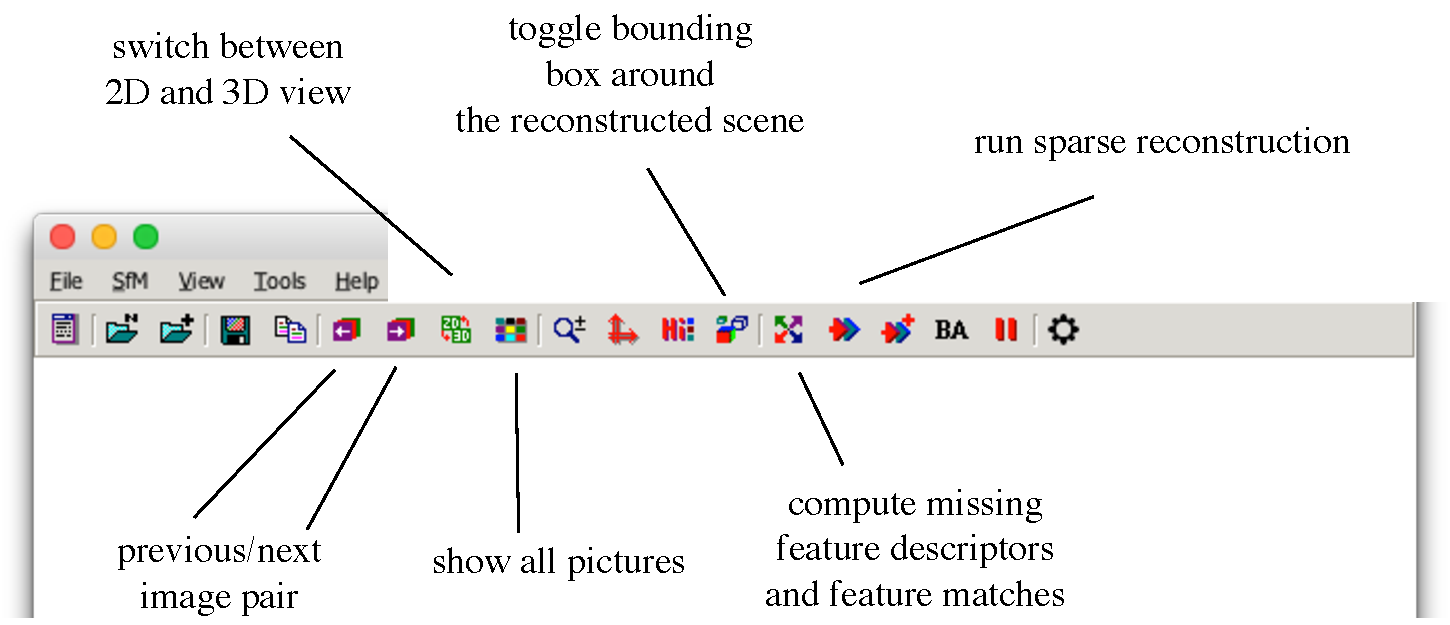
\includegraphics[keepaspectratio,width=\textwidth]{fig/visualsfm-gui.pdf}
	\end{center}
	\caption{GUI of the VisualSFM with few important buttons.}
	\label{fig:visualsfm-gui}
\end{figure}
\section{Reconstruction Process}
The whole process of reconstruction follows:
\begin{itemize}
	\item[1.] Choose \textbf{File} $\rightarrow$ \textbf{Open+ Multi Images}, navigate yourself to the dataset and select desired photos. After a while the photos should load into the system and should be displayed in a matrix.
	\item[2.] Next we need to compute keypoints and feature correspondences. Click 
\includegraphics[keepaspectratio,width=.5cm]{fig/visualsfm-compute-matches.png} or choose \textbf{SfM} $\rightarrow$ \textbf{Pairwise Matching} $\rightarrow$ \textbf{Compute Missing Match}. The system will now detect keypoints and calculate matches for all new photos. These feature and matches are implicitly cached in separate files \texttt{.sift} and \texttt{.mat}. Please note that this step may take a significant amount of time. The progress is shows in the \textbf{Log Window}.
	\item[3.] Click on the button 
\includegraphics[keepaspectratio,width=.5cm]{fig/visualsfm-sparse-reconstruction.png} or choose \textbf{SfM} $\rightarrow$ \textbf{Reconstruct Sparse} to compute sparse reconstruction. The view should change slightly showing the reconstructed 3D scene. The program may not create single model for the input dataset, but you can browse distinct models by pressing up and down arrow keys (model number is indicated in the window name between first pair of square brackets).
	\item[4.] Last step is running the dense reconstruction. Click 
\includegraphics[keepaspectratio,width=.5cm]{fig/visualsfm-dense-reconstruction.png} or choose \textbf{SfM} $\rightarrow$ \textbf{Reconstruct Dense}. You will be prompted to choose working directory and once all the files are saved to this directory, the PMVS2 dense reconstruction starts. Note that the dense reconstruction is a complex problem and takes a lot of time. Once finished, you can toggle between sparse and dense with hotkey \textbf{tabulator}. An example of sparse and dense reconstruction is in the figure \ref{fig:visualsfm-sparse-dense}.
\end{itemize}
The output, dense structure of each model is stored in folder \texttt{models} in a PLY format. The estimated camera calibrations can be found in the text file \texttt{cameras\textunderscore v2.txt}. The camera centres are stored in the PLY format as  \texttt{centers-[model\textunderscore ID].ply} containing the 3D locations for every camera in each model.
\begin{figure}[h]
	\begin{center}
		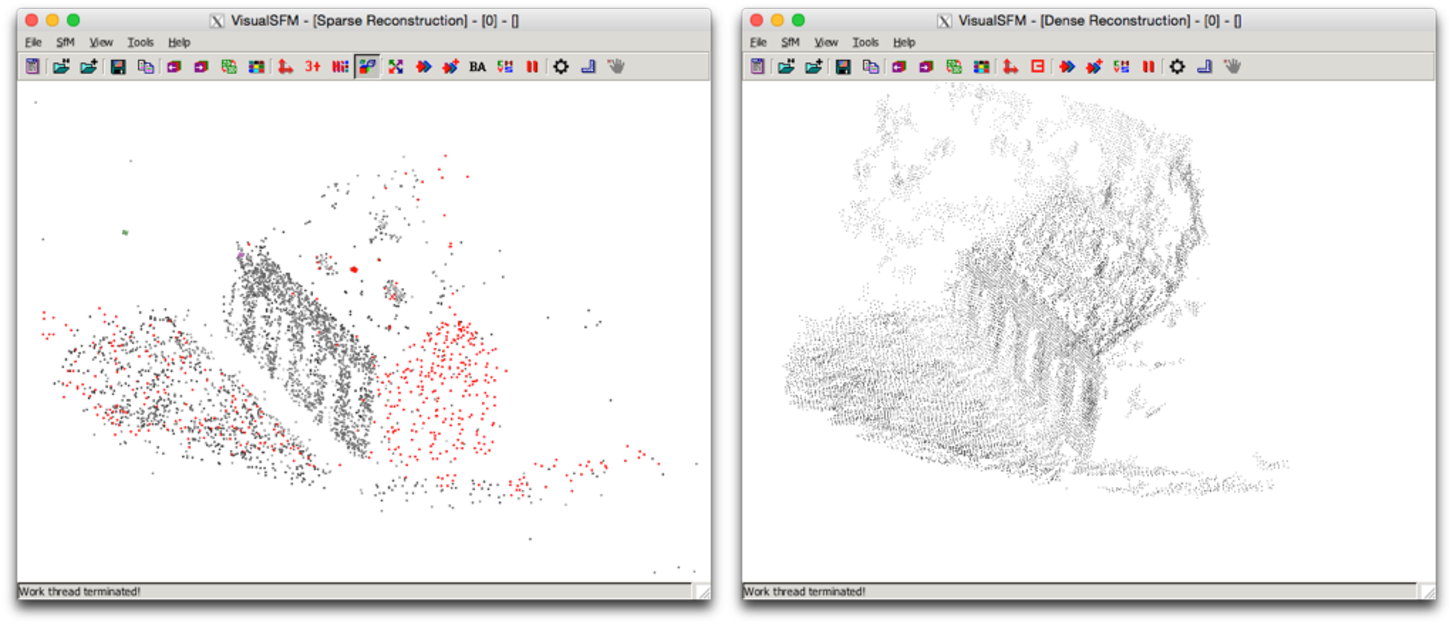
\includegraphics[keepaspectratio,width=\textwidth]{fig/visualsfm-sparse-dense.pdf}
	\end{center}
	\caption{Sparse (left) and dense (right) reconstruction of the Model House dataset.}
	\label{fig:visualsfm-sparse-dense}
\end{figure}

\section{Useful Tips and Controls}
The VisualSFM offers many hidden functionality useful for reconstructing the 3D scene. Full list can be found in the VisualSfM online documentation\footnote{VisualSfM documentation \url{http://ccwu.me/vsfm/doc.html}}.
\begin{itemize}
	\item \textbf{Camera calibration.} If camera calibration is known, it can be provided to the program by choosing \textbf{SfM} $\rightarrow$ \textbf{More Functions} $\rightarrow$ \textbf{Set Fixed Calibration}. This calibration can be also made shared across all cameras.
	
	\item \textbf{Selecting Initial Pair.} Initial camera pair for the reconstruction can be chosen by selecting the pair with left and right arrow keys and then choosing \textbf{SfM} $\rightarrow$ \textbf{More Functions} $\rightarrow$ \textbf{Set Initialization Pair}.
	
	\item \textbf{Keyboard shortcuts and mouse controls.}
	
	\begin{tabular}{l l}
		\textbf{Mouse middle wheel} & Zoom the scene. \\
		\textbf{Right mouse drag} & Rotate the scene. \\
		\textbf{Left mouse drag} & Pan the scene. \\
		\textbf{Tabulator} & Switch between sparse and dense reconstruction. \\
		\textbf{Up/Down} & Switch between different models. \\
		\textbf{Left/Right} & Switch between camera pairs. \\
		\textbf{T} & Switch between visualization modes: \begin{tabular}{l}
			\text{1) cameras + 3D points} \\
			\text{2) cameras only} \\
			\text{3) 3D points only} \\
		\end{tabular}\\
	\end{tabular}
\end{itemize}

\chapter{Dense to Textured Surface Reconstruction using Meshlab and Blender}
\label{app:surface-reconstruction}
This chapter describes the process of creation textured 3D polygonal model from dense point cloud. It assume that the user have a 3D dense reconstruction in a format produced by VisualSFM. The process start in MeshLab:
\begin{itemize}
	\item[1.] In MeshLab, select \textbf{File} $\rightarrow$ \textbf{OpenProject} and choose file \texttt{bundle.rd.out} in the dense reconstruction data folder. Next prompt requires the \texttt{list.txt} from the same folder. 
	\item[2.] Right now the sparse point cloud is opened which is not what we want. Click the icon 
\includegraphics[keepaspectratio,width=.5cm]{fig/meshlab-layers.png} or \textbf{View} $\rightarrow$ \textbf{Show Layer Dialog}. A new toolbar will appear on the right of the screen. Click on the model with the right mouse button and from the context menu select \textbf{Delete Current Mesh} (as depicted in figure \ref{fig:meshlab-1}).
\begin{figure}[h]
	\begin{center}
		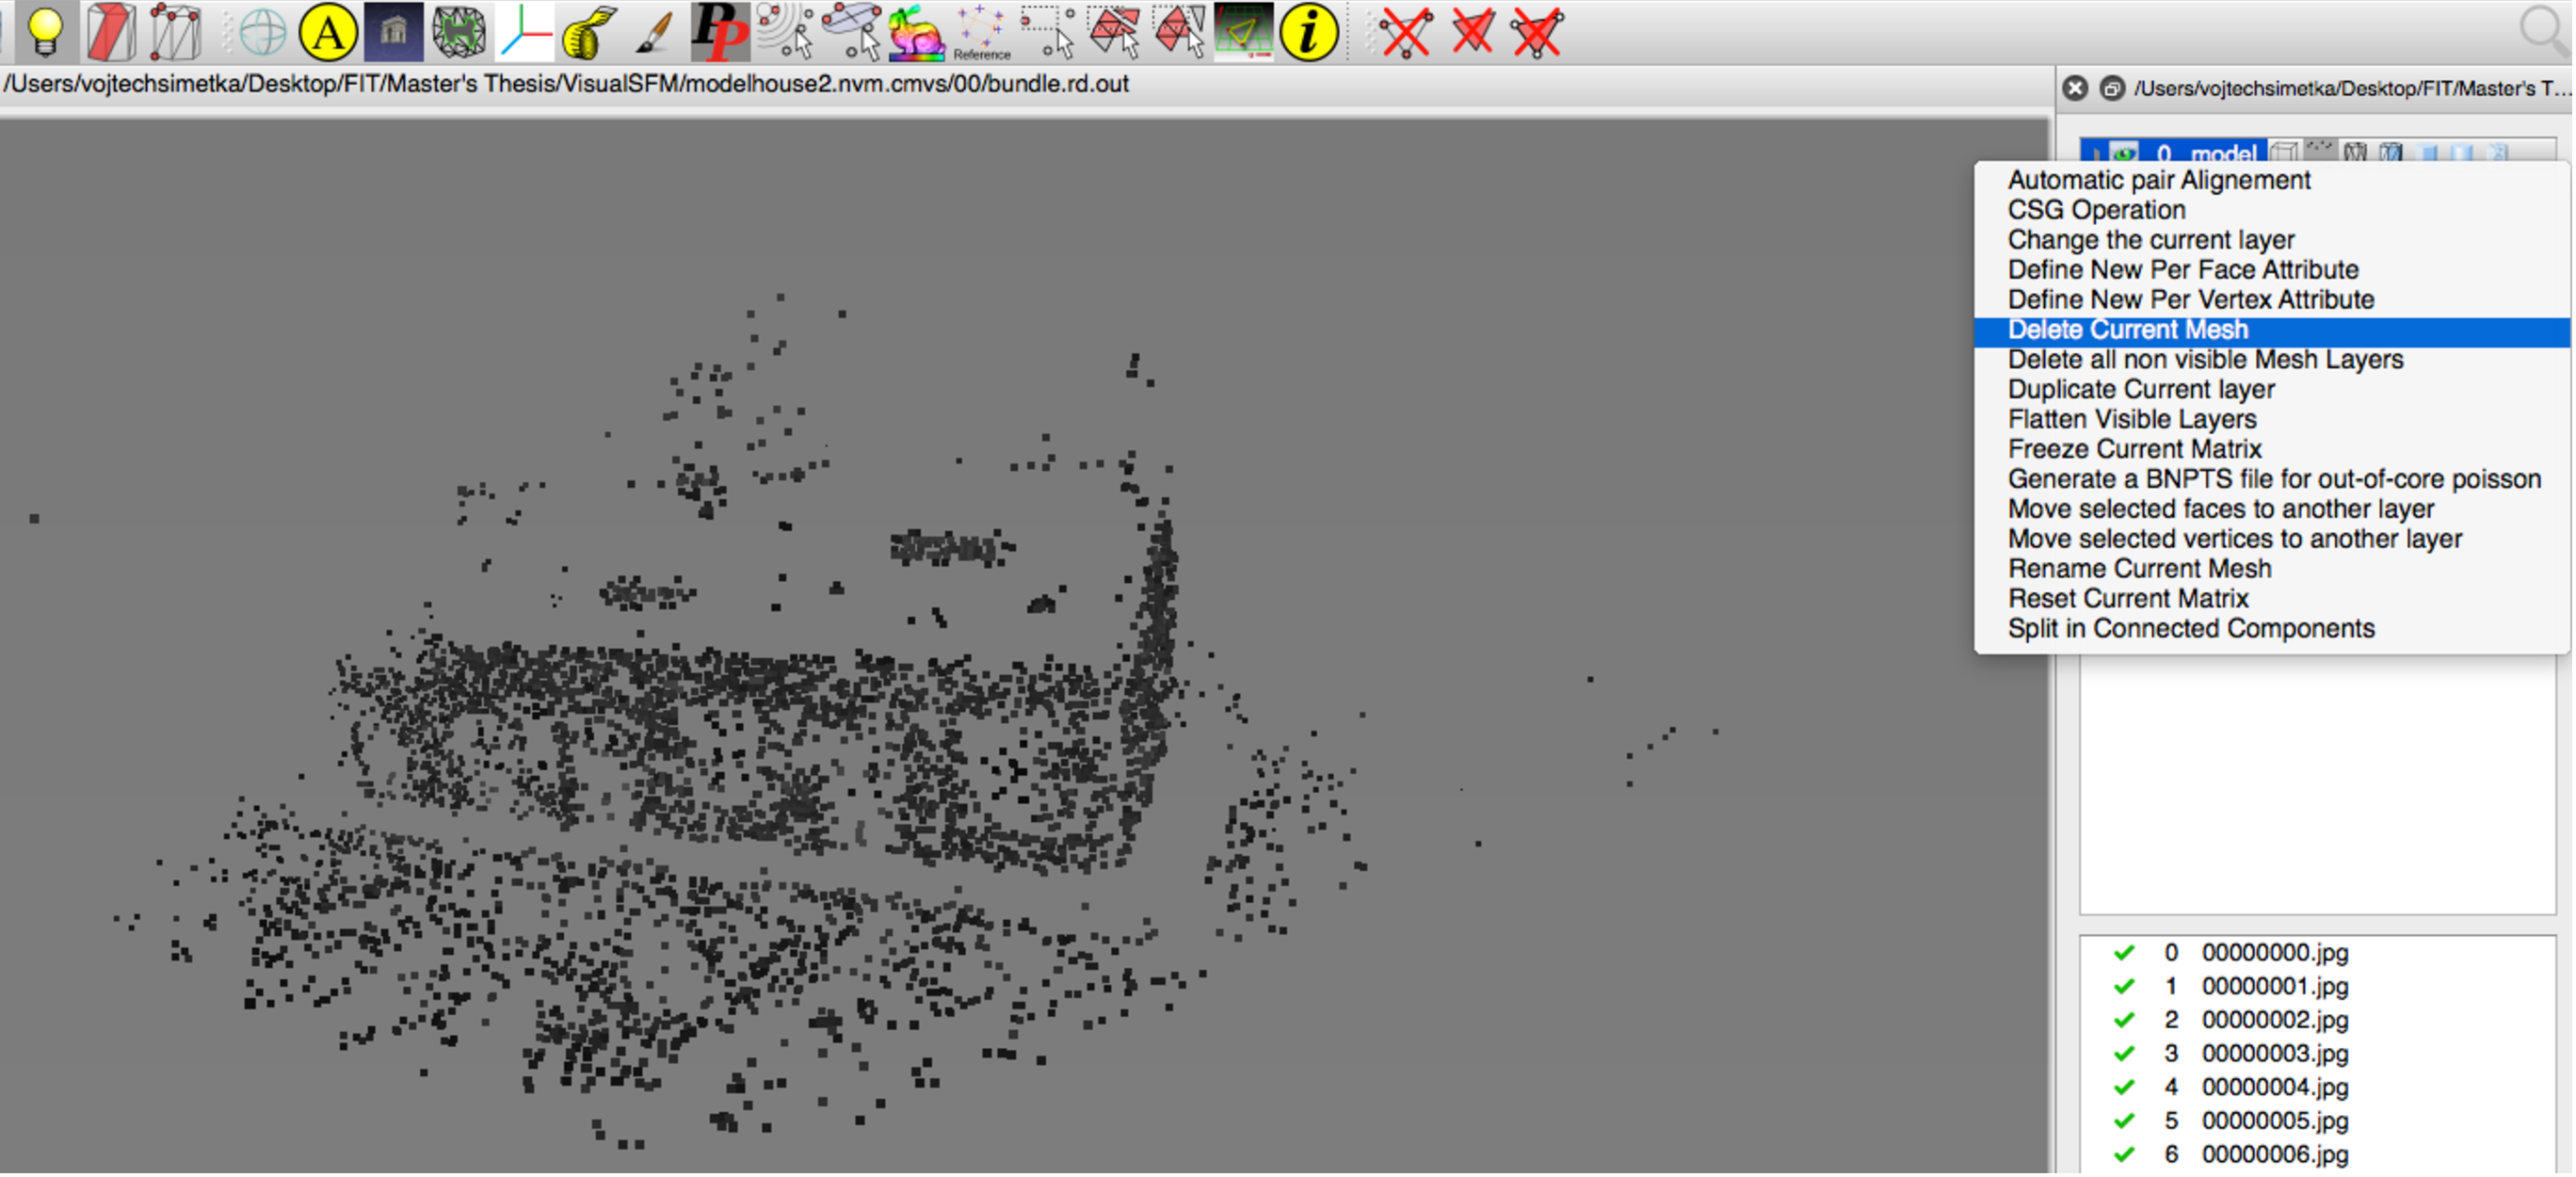
\includegraphics[keepaspectratio,width=9cm]{fig/meshlab-1.pdf}
	\end{center}
	\caption{How to erase sparse cloud mesh in MeshLab.}
	\label{fig:meshlab-1}
\end{figure}
	\item[3.] Choose \textbf{File} $\rightarrow$ \textbf{Import Mesh} and select adequate model from folder \texttt{models}.
	\item[4.] The model shown is now a dense point cloud, but it is almost certainly quite noisy. We can remove some of the noisy data by selecting them with tool 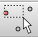
\includegraphics[keepaspectratio,width=.5cm]{fig/meshlab-select.png} (\textbf{Edit} $\rightarrow$ \textbf{Select Vertices}), and erasing them with 
\includegraphics[keepaspectratio,width=.5cm]{fig/meshlab-delete.png}.

	\item[5.] Next step is to create a surface reconstruction. Choose \textbf{Filters} $\rightarrow$ \textbf{Point Set} $\rightarrow$ \textbf{Surface Reconstruction: Poisson}. We suggest you to use following values:
	
	\begin{tabular}{l l}
		Octree Depth & 12 \\
		Solver Divide & 10 \\
		Samples per Node & 1 \\
		Surface offsetting & 1 \\
	\end{tabular}
	
%\begin{figure}[ht]
%	\begin{center}
%		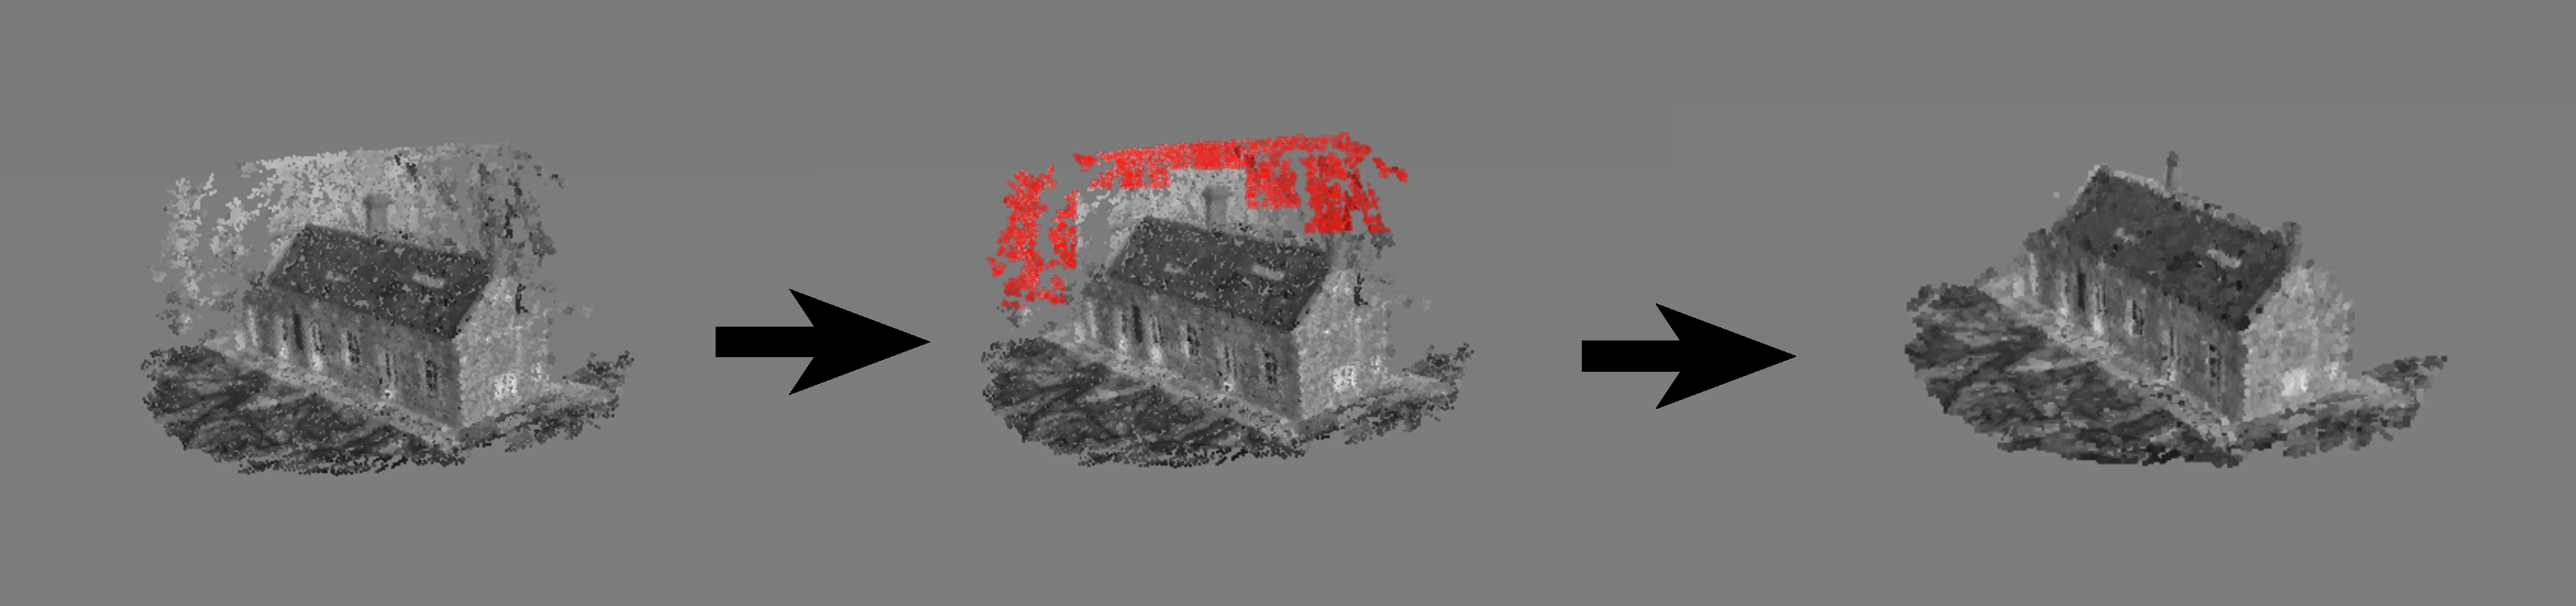
\includegraphics[keepaspectratio,width=\textwidth]{fig/meshlab-2.pdf}
%	\end{center}
%	\caption{The process of manually erasing incorrect points.}
%	\label{fig:meshlab-2}
%\end{figure}

	\item[6.] However, the surface reconstruction creates a lots of incorrect faces. We once again erase the vertices using tools from step 4. Once done, choose \textbf{Filters} $\rightarrow$ \textbf{Selection} $\rightarrow$ \textbf{Select non-manifold Edges}, hit apply and erase these points with vertex erase tool 
\includegraphics[keepaspectratio,width=.5cm]{fig/meshlab-delete.png}.
	
	\item[7.] Now we finally apply textures. Select \textbf{Filters} $\rightarrow$ \textbf{Texture} $\rightarrow$ \textbf{Parametrization + texturing from registered rasters}. Make sure the following options are checked: \textbf{Color correction, Use distance weight, Use image border weight, Clean isolated triangles} and \textbf{UV stretching}.
	\item[8.] The last step in the MeshLab tool is to export the model to the file format supported by Blender. Select \textbf{File} $\rightarrow$ \textbf{Export mesh as} and make sure you save it as an \texttt{obj} type.
\end{itemize}

The next part is more or less optional and contains mostly just storing the texture in the file itself.
\begin{itemize}
	\item[1.] Lets open Blender, right click on the cube, hit key \textbf{x} and click delete.
	\item[2.] Choose \textbf{File} $\rightarrow$ \textbf{Import} $\rightarrow$ \textbf{Wavefront (.obj)}.
	\item[3.] On the panel on the right select texture tab. Add new texture and change the type of the texture to \textbf{Image or Movie}. Ten press \textbf{Open} and load the appropriate texture file. If necessary the UV mapping coordinates can be altered, but this is beyond the scope of our tutorial.
	\item[4.] Now we can export the 3D model to some reasonable 3D file format, for example the\texttt{fbx}.
\end{itemize} 


\begin{figure}[ht]
	\begin{center}
		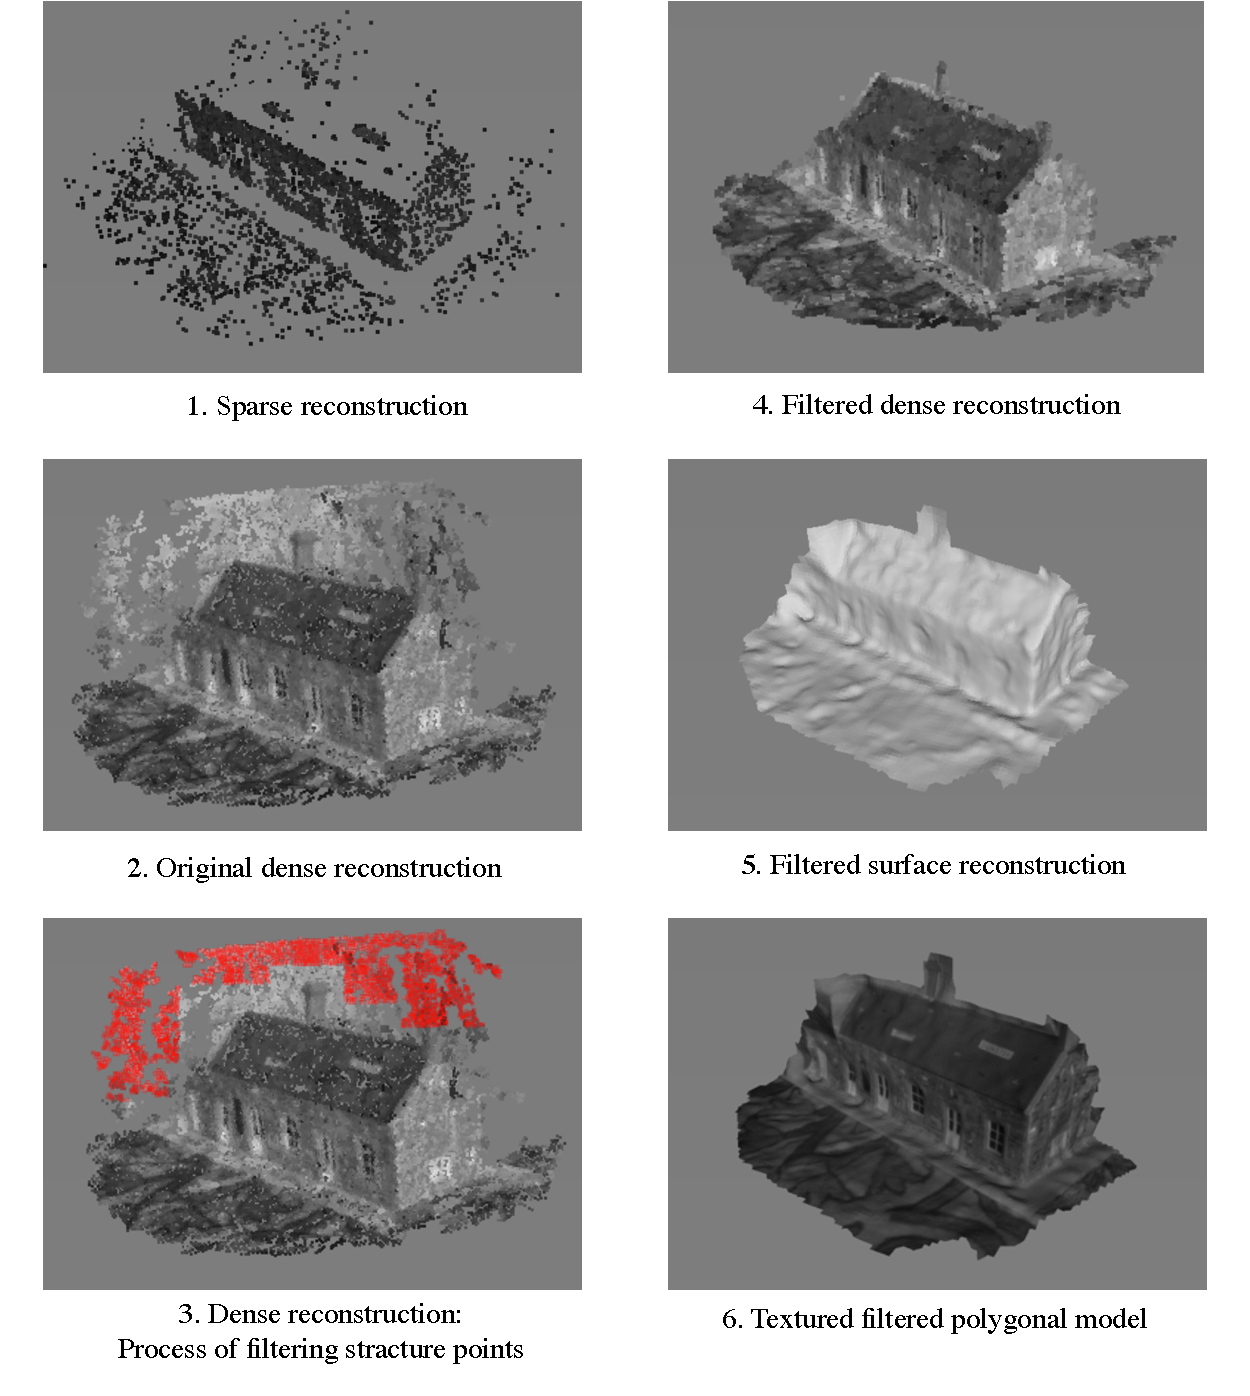
\includegraphics[keepaspectratio,width=\textwidth]{fig/reconstruction-overview.pdf}
	\end{center}
	\caption{Distinct reconstruction phases from sparse reconstruction to textured 3D model.}
	\label{fig:reconstruction-overview}
\end{figure}

%\chapter{Manual}
%\chapter{Konfigrační soubor}
%\chapter{RelaxNG Schéma konfiguračního soboru}
%\chapter{Plakat} % viz. prilohy.tex
\end{document}
